\documentclass[8pt,aspectratio=1610]{beamer}
\usepackage{units,multicol,booktabs,tikz,xparse,tikz-3dplot,mathtools,url}
\usepackage[labelformat=empty]{caption}
\usetikzlibrary{arrows.meta,calc,shapes,angles,quotes,patterns}

\usepackage[square,comma,sort,numbers]{natbib}
\bibliographystyle{plainnat} % nat styles allow urls in bib

% as links are in footer, best to use url package and modify colors as here
\renewcommand\UrlFont{\color{blue!50!black}} 

% allows to not count appendix slides in slide number
\usepackage{appendixnumberbeamer} 

%\hypersetup{colorlinks, linkcolor={blue!50!black}, citecolor={red!70!black}, urlcolor={blue!50!black}}
\graphicspath{{Images/}}
%Display framenumber in footer
\newcommand*\oldmacro{}%
\let\oldmacro\insertshorttitle%
\renewcommand*\insertshorttitle{%
  \oldmacro\hfill%
  \insertframenumber\,/\,\inserttotalframenumber}

%Choose colors for themes
\definecolor{myblue}{rgb}{0.2,0.2,0.7} %Default Warsaw
\definecolor{myred}{RGB}{165,8,8}
\definecolor{myviolet}{RGB}{100,8,165}
\definecolor{mygreen}{RGB}{0,132,15}

%Tikz colors
\definecolor{bluegrid}{RGB}{197,207,224}

% Initialize default color theme
\setbeamercolor{author in head/foot}{bg=black} 		%1501 foot
\setbeamercolor{subsection in head/foot}{bg=myblue} 	% lecture title foot
\setbeamercolor{section in head/foot}{bg=black} 		% frametitle gradient
\setbeamercolor{frametitle}{bg=myblue} 				%frametitle primary color
\setbeamercolor{local structure}{fg=black}				%Necessary for enumerate
\setbeamercolor{item projected}{bg=myblue}			%itemize bullets

% iClicker enumerate box drawing
\newcommand{\tikzmark}[1]{\tikz[overlay,remember picture] \node (#1) {};}

% Macros
\newcommand{\vect}[1]{\mathbf{#1}}
\newcommand{\vecth}[1]{\hat{\mathbf{#1}}}
\def\flb#1\fle{\begin{flalign*}#1\end{flalign*}} % begin / end full left align

% More Stuff
\usefonttheme[onlymath]{serif}
\setbeamercovered{invisible}
\hfuzz=60pt %Surpresses hbox full warnings by extending to 50pt
\newdimen\hfuzz
\vbadness = 10000 %Similar to hbox warning supression

% Mode
\mode<presentation>{\usetheme{Warsaw}}

% Prevent new section being generated from bibliography
\renewcommand{\bibsection}{}

% Generate Credentials
\title[Cosmological Fluctuations]{Cosmological Fluctuations in Standard and Conformal Gravity}
\author[Matthew Phelps]{Matthew Phelps}
\institute{\normalsize{Doctoral Degree Final Examination}
\and 
\includegraphics[width=0.8 in]{uconn-logo.png} }
\date{June 02, 2020}


%%%%%%%%%%%%%%%%%%%%%%%%%%%%%%%%%%%%%%%%%%%%%%%%%%%%%%%%%%%%%%
% Begin Document
%%%%%%%%%%%%%%%%%%%%%%%%%%%%%%%%%%%%%%%%%%%%%%%%%%%%%%%%%%%%%%
%\includeonlyframes{current}

\begin{document}
\beamertemplatenavigationsymbolsempty %Remove navigation icons
\setbeamertemplate{enumerate item}{(\Alph{enumi})} %Set default enumeration style


%%%%%%%%%%%%%%%%%%%%%%%%%%%%%%%%%%%%%%%%%%%%%%%%%%%%%%%%%%%%%%
% Slide  - Background Slide
%%%%%%%%%%%%%%%%%%%%%%%%%%%%%%%%%%%%%%%%%%%%%%%%%%%%%%%%%%%%%%

%\begingroup
%\Large
%\begin{frame}[plain]
%        \begin{tikzpicture}[remember picture,overlay]
%\node[at=(current page.center)] {
%	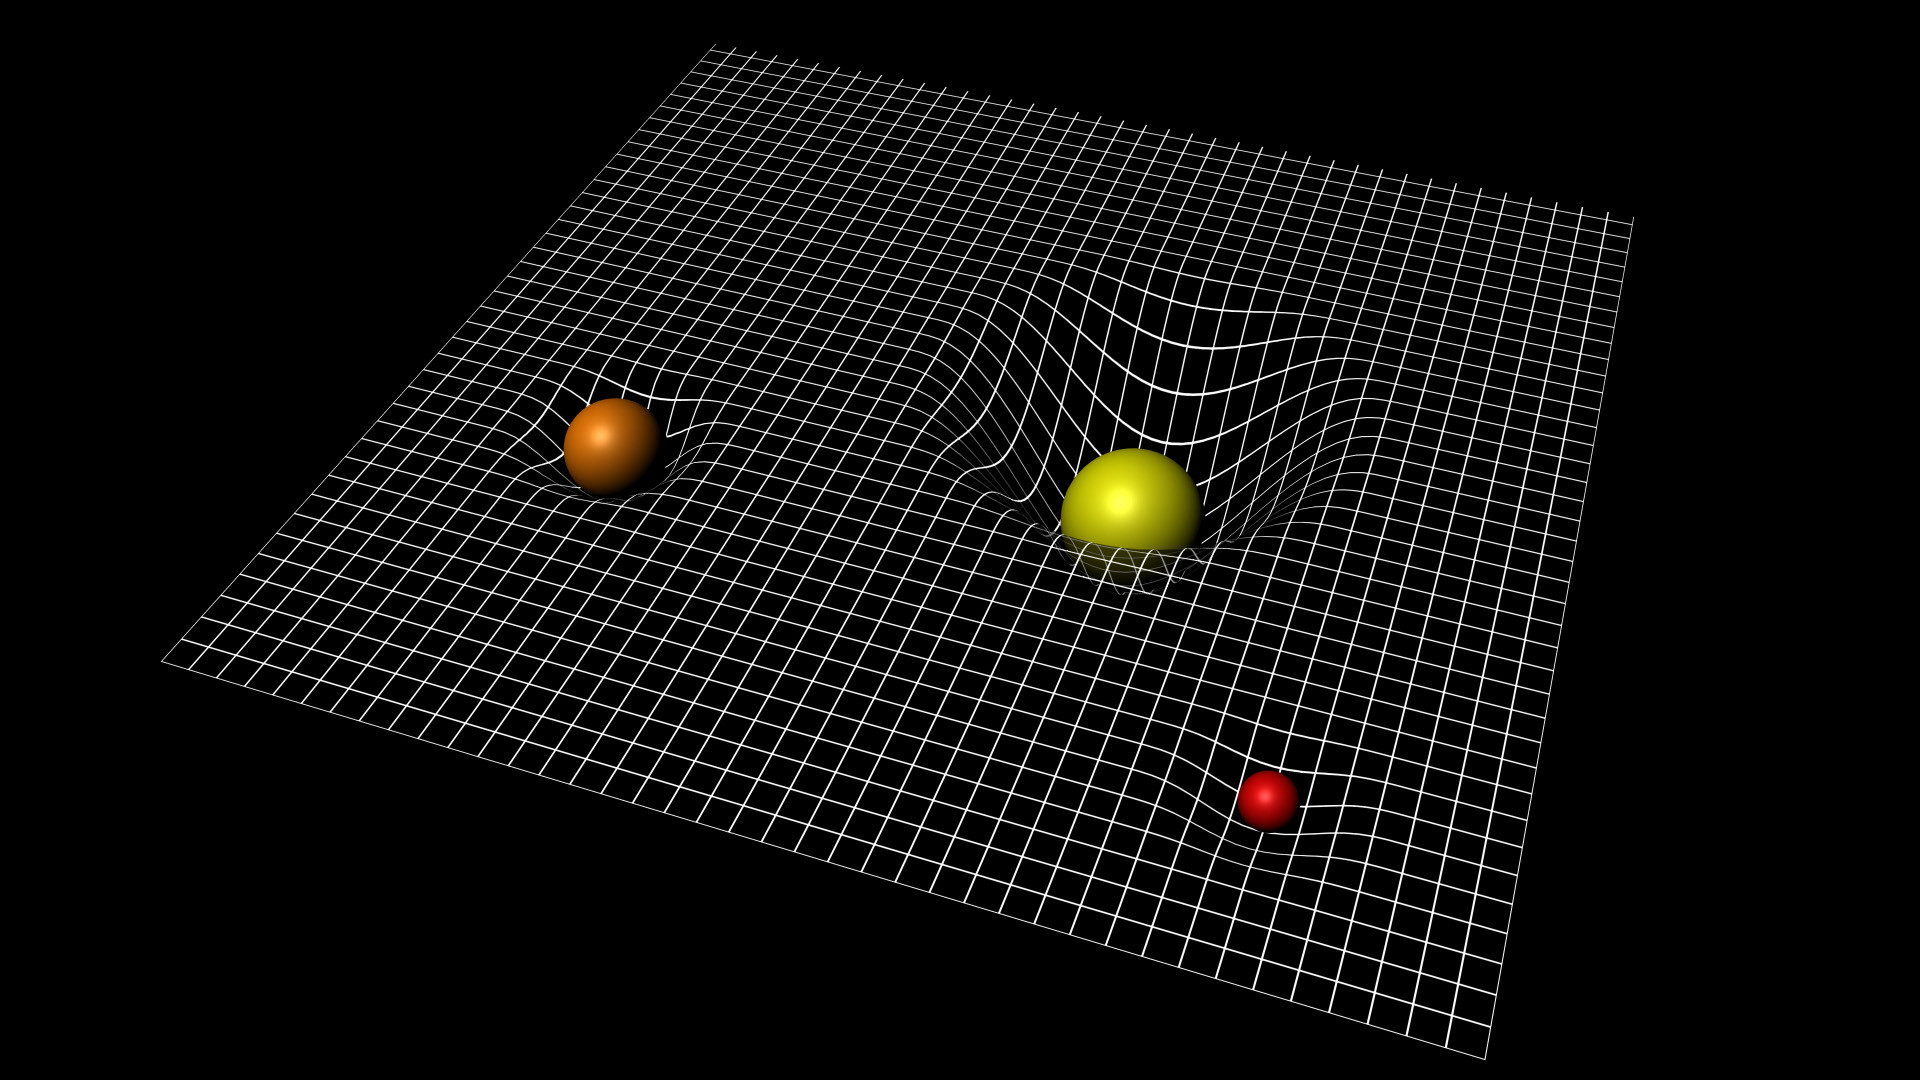
\includegraphics[width=\paperwidth]{spacetime_curvature.jpg}
%};
%\end{tikzpicture}
%\end{frame}
%\endgroup


%%%%%%%%%%%%%%%%%%%%%%%%%%%%%%%%%%%%%%%%%%%%%%%%%%%%%%%%%%%%%%
% Slide  - Title Page
%%%%%%%%%%%%%%%%%%%%%%%%%%%%%%%%%%%%%%%%%%%%%%%%%%%%%%%%%%%%%%

\begingroup
\Large
\begin{frame}
\setcounter{framenumber}{0}
	\titlepage
\end{frame}
\endgroup

%%%%%%%%%%%%%%%%%%%%%%%%%%%%%%%%%%%%%%%%%%%%%%%%%%%%%%%%%%%%%%
% Slide  - TOC
%%%%%%%%%%%%%%%%%%%%%%%%%%%%%%%%%%%%%%%%%%%%%%%%%%%%%%%%%%%%%%

\begingroup
\Large
\begin{frame}{Overview}
	\begin{itemize}
		\item Introduction and Formalism
		\item Three Dimensional Scalar, Vector, Tensor Decomposition (SVT3)
		\item Four Dimensional Scalar, Vector, Tensor Decomposition (SVT4)
		\item Conformal Gravity (SVT and Conformal to Flat Backgrounds)
		\item Conformal Gravity Robertson-Walker Radiation Era Solution
		\item Conclusions
		\item Computational Methods
	\end{itemize}
\end{frame}
\endgroup

%%%%%%%%%%%%%%%%%%%%%%%%%%%%%%%%%%%%%%%%%%%%%%%%%%%%%%%%%%%%%%
% Slide  - Introduction and Formalism
%%%%%%%%%%%%%%%%%%%%%%%%%%%%%%%%%%%%%%%%%%%%%%%%%%%%%%%%%%%%%%

%\begingroup
%\Large
%\begin{frame}{Introduction and Formalism Overview}
%	\begin{itemize}
%		\item Introduction and Formalism
%		\begin{itemize}
%			\large{
%			\item Cosmological Geometries
%			\item Einstein Gravity
%			\item Perturbation Theory
%			\item Gauge Transformations
%			\item Solution Methods
%			}
%		\end{itemize}
%	\end{itemize}
%\end{frame}
%\endgroup

%%%%%%%%%%%%%%%%%%%%%%%%%%%%%%%%%%%%%%%%%%%%%%%%%%%%%%%%%%%%%%
% Slide  - Cosmological Geometries 
%%%%%%%%%%%%%%%%%%%%%%%%%%%%%%%%%%%%%%%%%%%%%%%%%%%%%%%%%%%%%%

\begin{frame}{Cosmological Geometries}
	\begin{columns}
	\begin{column}{0.5\linewidth}
	\begin{itemize}
		\item Cosmological Principle: Structure of spacetime is homoegenous and isotropic at large scales
		\item Geometries: Robertson Walker (flat, spherical, hyperbolic), de Sitter ($dS_4 \subset \rm{RW}$)
		\item All background geometries relevant to cosmology can be expressed as conformal to flat
	\begin{eqnarray*}
		ds^2 = \Omega(x)^2\big(-dt^2 + dx^2 + dy^2 + dz^2\big)
	\end{eqnarray*}
	\end{itemize}
	\end{column}
	\begin{column}{0.5\linewidth}
		\begin{figure}
			\includegraphics[width=\linewidth]{hubble_deep.jpg}
			{\caption*{Hubble Ultra-Deep Field. NASA and the European Space Agency.}}
		\end{figure}
	\end{column}
	\end{columns}
\end{frame}

%%%%%%%%%%%%%%%%%%%%%%%%%%%%%%%%%%%%%%%%%%%%%%%%%%%%%%%%%%%%%%
% Slide  - Cosmological Geometries R.W. k=0
%%%%%%%%%%%%%%%%%%%%%%%%%%%%%%%%%%%%%%%%%%%%%%%%%%%%%%%%%%%%%%

\begin{frame}{Cosmological Geometries R.W.}
	\begin{itemize}
		\item Comoving Robertson Walker geometry:
		\begin{eqnarray}
		ds^2 &=& -dt^2 + a(t)^2 \tilde g_{ij}dx^i dx^j
		\nonumber\\
		&=& -dt^2 + a(t)^2\bigg[\frac{dr^2}{1-kr^2} + r^2 d\theta^2 + r^2 \sin^2\theta d\phi^2\bigg]
		\end{eqnarray}
		\item 3-Space Curvature Tensors,
		\begin{eqnarray}
		R_{ijkl} = k(\tilde g_{jk}\tilde g_{il} - \tilde g_{ik}\tilde g_{jl}), \qquad R_{ij} = -2k\tilde g_{ij}, \qquad R = -6k,\qquad k \in \{-1,0,1\}
		\end{eqnarray}
		\item Define the conformal time
		\begin{eqnarray}
		\tau = \int \frac{dt}{a(t)},
		\end{eqnarray}
	\end{itemize}
	\only<1>{
	\begin{eqnarray}
		ds^2 = a(\tau)^2\bigg[-d\tau^2 + \frac{dr^2}{1-kr^2} + r^2 d\theta^2 + r^2 \sin^2\theta d\phi^2\bigg]
	\end{eqnarray}
	}
	\only<2>{
	\begin{itemize}
		\item Set $k=0$ (flat), simple conformal to flat form
	\end{itemize}
	\begin{eqnarray}
		\boxed{ds^2 = a(\tau)^2\bigg[-d\tau^2 + dr^2 + r^2 d\theta^2 + r^2 \sin^2\theta d\phi^2\bigg]}
	\end{eqnarray}		
	}
\end{frame}

%%%%%%%%%%%%%%%%%%%%%%%%%%%%%%%%%%%%%%%%%%%%%%%%%%%%%%%%%%%%%%
% Slide  - Cosmological Geometries R.W. k=1
%%%%%%%%%%%%%%%%%%%%%%%%%%%%%%%%%%%%%%%%%%%%%%%%%%%%%%%%%%%%%%

\begin{frame}{Cosmological Geometries R.W. $k=1$}
	\begin{itemize}
		\item $k=1$ (spherical)
		\begin{eqnarray}
		ds^2 = a(\tau)^2\bigg[-d\tau^2 + \frac{dr^2}{1-r^2} + r^2 d\theta^2 + r^2 \sin^2\theta d\phi^2\bigg]
		\end{eqnarray}
		\item Set $\sin\chi = r$, $p = \tau$,
		\begin{eqnarray}
		ds^2 = a(p)^2\bigg[-dp^2 + d\chi^2 + \sin^2\chi d\theta^2 + \sin^2\chi \sin^2\theta d\phi^2\bigg]
		\end{eqnarray}
		\item Introduce coordinates
		\begin{eqnarray}
		p' + r' &=& \tan[(p+\chi)/2],\quad p'-r'=\tan[(p-\chi)/2]
		\nonumber\\
		p' &=& \frac{\sin p}{\cos p + \cos \chi}, \quad r' = \frac{\sin\chi}{\cos p + \cos\chi}
		\end{eqnarray}
		\begin{eqnarray}
		\implies \boxed{ds^2 = \frac{4a^2(p)}{[1+(p'+r')^2][1+(p'-r')^2]}[-dp'^2 + dr'^2 +r'^2 d\theta^2 + r'^2\sin^2\theta d\phi^2]}
		\end{eqnarray}
	\end{itemize}
\end{frame}

%%%%%%%%%%%%%%%%%%%%%%%%%%%%%%%%%%%%%%%%%%%%%%%%%%%%%%%%%%%%%%
% Slide  - Cosmological Geometries R.W. k=-1
%%%%%%%%%%%%%%%%%%%%%%%%%%%%%%%%%%%%%%%%%%%%%%%%%%%%%%%%%%%%%%

\begin{frame}{Cosmological Geometries R.W. $k=-1$}
	\begin{itemize}
		\item $k=-1$ (hyperbolic) \textcolor{white}{\cite{phelps_2019}}\textcolor{white}{\cite{amarasinghe_2019}}
		\begin{eqnarray}
		ds^2 = a(\tau)^2\bigg[-d\tau^2 + \frac{dr^2}{1+r^2}  + r^2 d\theta^2 + r^2 \sin^2\theta d\phi^2\bigg]
		\end{eqnarray}
		\item Set $\sinh\chi = r$, $p = \tau$,
		\begin{eqnarray}
		ds^2 = a(p)^2\bigg[-dp^2 + d\chi^2 + \sinh^2\chi d\theta^2 + \sinh^2\chi \sin^2\theta d\phi^2\bigg]
		\end{eqnarray} 
		\item Introduce coordinates
		\begin{eqnarray}
		p' + r' &=& \tanh[(p+\chi)/2],\quad p'-r'=\tanh[(p-\chi)/2]
		\nonumber\\
		p' &=& \frac{\sinh p}{\cosh p + \cosh \chi}, \quad r' = \frac{\sinh\chi}{\cosh p + \cosh\chi}
		\end{eqnarray}
		\begin{eqnarray}
		\implies \boxed{ds^2 = \frac{4a^2(p)}{[1-(p'+r')^2][1-(p'-r')^2]}[-dp'^2 + dr'^2 +r'^2 d\theta^2 + r'^2\sin^2\theta d\phi^2]}
		\end{eqnarray}
	\end{itemize}
\end{frame}

%%%%%%%%%%%%%%%%%%%%%%%%%%%%%%%%%%%%%%%%%%%%%%%%%%%%%%%%%%%%%%
% Slide  - Einstein Gravity
%%%%%%%%%%%%%%%%%%%%%%%%%%%%%%%%%%%%%%%%%%%%%%%%%%%%%%%%%%%%%%

\begin{frame}{Einstein Gravity}
	\begin{itemize}
		\item 	Einstein Hilbert action
		\begin{eqnarray}
		I_{\text{EH}} = -\frac{1}{16\pi G} \int d^4x (-g)^{1/2}  g^{\mu\nu}R_{\mu\nu}
		\end{eqnarray}
		\item 	Functional variation w.r.t $g_{\mu\nu}$ yields Einstein tensor,
		\begin{eqnarray}
		\frac{16\pi G}{(-g)^{1/2}} \frac{\delta I_{\text{EH}}}{\delta g_{\mu\nu}}= G^{\mu\nu} = R^{\mu\nu} - \frac{1}{2}g^{\mu\nu}R^\alpha{}_\alpha
		\end{eqnarray}
		\item 	Likewise, variation of matter action $I_{\rm M}$ w.r.t $g_{\mu\nu}$ yields Energy Momentum tensor
		\begin{eqnarray}
		\frac{2}{(-g)^{1/2}} \frac{ \delta I_\text{M}}{\delta g_{\mu\nu}} = T_{\mu\nu}
		\end{eqnarray}
		\item 	Requiring sum of actions to be stationary gives us Einstein field equations
		\begin{eqnarray}
		R^{\mu\nu} - \frac{1}{2}g^{\mu\nu}R^\alpha{}_\alpha = -8\pi G T^{\mu\nu},
		\label{EinEOM}
		\end{eqnarray}
		subject to Bianchi identity
		\begin{eqnarray}
		\nabla_\mu R^{\mu\nu} = \frac{1}{2}\nabla^\nu R^\mu{}_\mu \implies \nabla_\mu G^{\mu\nu} = 0
		\end{eqnarray}
	\end{itemize}
\end{frame}

%%%%%%%%%%%%%%%%%%%%%%%%%%%%%%%%%%%%%%%%%%%%%%%%%%%%%%%%%%%%%%
% Slide  - Perturbation Theory
%%%%%%%%%%%%%%%%%%%%%%%%%%%%%%%%%%%%%%%%%%%%%%%%%%%%%%%%%%%%%%

\begin{frame}{Cosmological Perturbation Theory}
	\begin{columns}
		\begin{column}{0.7\linewidth}
			\begin{itemize}
			\item Introduce fluctuation to background $g_{\mu\nu}^{(0)}$
			\begin{eqnarray}
				g_{\mu\nu}(x) &=& g_{\mu\nu}^{(0)}(x) + h_{\mu\nu}(x),\qquad g^{\mu\nu}_{(0)}h_{\mu\nu} \equiv h
				\\ \nonumber\\
				G_{\mu\nu} &=& G_{\mu\nu}(g_{\mu\nu}^{(0)}) + \delta G_{\mu\nu}(h_{\mu\nu})
				\\ \nonumber\\
				G_{\mu\nu}^{(0)} &=& R_{\mu\nu}^{(0)} -\frac{1}{2} g_{\mu\nu}^{(0)} R_\alpha^{(0)\alpha}
				\label{Einzero}
				\\ \nonumber\\
				\delta G_{\mu\nu} &=& \delta R_{\mu\nu} - \frac{1}{2} h_{\mu\nu} R_\alpha^{(0)\alpha} -\frac{1}{2}g_{\mu\nu}\delta R^\alpha{}_\alpha.
			\end{eqnarray}
			\item Likewise perturb $T_{\mu\nu}$
			\begin{eqnarray}
				T_{\mu\nu} &=& T_{\mu\nu}(g_{\mu\nu}^{(0)}) + \delta T_{\mu\nu}(h_{\mu\nu})
			\end{eqnarray}
			\item Form background and first order equations of motion
			\end{itemize}
		\end{column}
		\begin{column}{0.3\linewidth}
			\begin{figure}[t]
				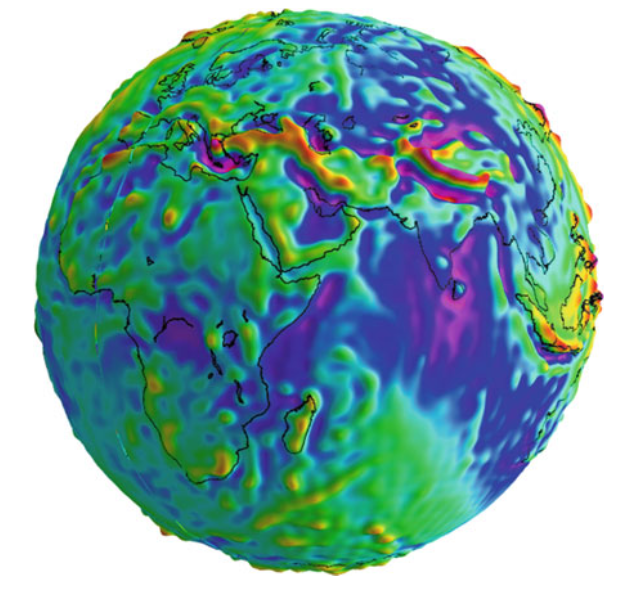
\includegraphics[width=\linewidth]{sphere_perturb.png}
			\end{figure}
			%\footnotemark
		\end{column}
	\end{columns}
		\begin{eqnarray}
		\Delta_{\mu\nu}^{(0)} &=& G_{\mu\nu}^{(0)} + T_{\mu\nu}^{(0)} =0
		\\
		\Delta_{\mu\nu} &=& \delta G_{\mu\nu}(h_{\mu\nu}) + \delta T_{\mu\nu}(h_{\mu\nu})=0
		\end{eqnarray}
		\let\thefootnote\relax\footnotetext{Walter, U. (2019). Correction to: Astronautics. In Astronautics (pp. C1–C1). Springer International Publishing.}
\end{frame}

%%%%%%%%%%%%%%%%%%%%%%%%%%%%%%%%%%%%%%%%%%%%%%%%%%%%%%%%%%%%%%
% Slide  - Gauge Transformations
%%%%%%%%%%%%%%%%%%%%%%%%%%%%%%%%%%%%%%%%%%%%%%%%%%%%%%%%%%%%%%

\begin{frame}{Gauge Transformations}
	\begin{itemize}
		\item Coordinate invariance $x^\mu \to x'^\mu$
		\begin{eqnarray}
			g'_{\mu\nu} = \frac{\partial x^\alpha}{\partial x'^\mu}\frac{\partial x^\beta}{\partial x'^\nu}g_{\alpha\beta}
		\end{eqnarray}
		\item 	Under coordinate transformation $x^\mu \to x^\mu - \epsilon^\mu(x)$, with $\nabla_\mu \epsilon_\nu \sim \mathcal O(h)$
			\begin{eqnarray}
				g'_{\mu\nu} &=& g_{\mu\nu} + \nabla_\mu \epsilon_\nu + \nabla_\nu \epsilon_\mu
				\\ \nonumber\\
				g^{(0)}_{\mu\nu} + h'_{\mu\nu} &=& g^{(0)}_{\mu\nu} + h_{\mu\nu} + \nabla_\mu \epsilon_\nu + \nabla_\nu \epsilon_\mu
				\\
				h_{\mu\nu} &\to& h_{\mu\nu} + \nabla_\mu \epsilon_\nu + \nabla_\nu \epsilon_\mu
				\\ \nonumber\\
				\delta G_{\mu\nu} &\to& \delta G_{\mu\nu} + {}^{(0)}G^\lambda{}_\mu \nabla_\nu \epsilon_\lambda +  {}^{(0)}G^{\lambda}{}_{\nu}\nabla_\mu \epsilon_\mu + \nabla_\lambda  G^{(0)}_{\mu\nu} \epsilon^\lambda
				\\ \nonumber\\
				\delta T_{\mu\nu} &\to& \delta T_{\mu\nu} + {}^{(0)}T^\lambda{}_\mu \nabla_\nu \epsilon_\lambda +  {}^{(0)}T^{\lambda}{}_{\nu}\nabla_\mu \epsilon_\mu + \nabla_\lambda  T^{(0)}_{\mu\nu} \epsilon^\lambda.
			\end{eqnarray}
		\item 	For every solution $h_{\mu\nu}$ to $\delta G_{\mu\nu} + \delta T_{\mu\nu} = 0$, a transformed $h'_{\mu\nu} = h_{\mu\nu} + \nabla_\mu \epsilon_\nu + \nabla_\nu \epsilon_\mu$ will also serve as a solution
		%\item Set of four $\epsilon^\mu(x)$ define gauge freedom under coordinate transformation
		%\item 10 components in $h_{\mu\nu}$, 4 coordinate transformations, leads to 6 independent degrees of freedom
		%\item If background $G_{\mu\nu}^{(0)} = 0$ , then $\delta G_{\mu\nu}$ separately gauge invariant; likewise for vanishing background energy momentum tensor
		%\item If $G_{\mu\nu}^{(0)} \ne 0$, then only the entire $\Delta_{\mu\nu} = \delta G_{\mu\nu} + T_{\mu\nu}$ is gauge invariant
	\end{itemize}


\end{frame}

%%%%%%%%%%%%%%%%%%%%%%%%%%%%%%%%%%%%%%%%%%%%%%%%%%%%%%%%%%%%%%
% Slide  - Solving Equations of Motion
%%%%%%%%%%%%%%%%%%%%%%%%%%%%%%%%%%%%%%%%%%%%%%%%%%%%%%%%%%%%%%

\begin{frame}{Solution Methods}
	%\begin{itemize}
		%\item Perturbed field equations $\delta G_{\mu\nu} + \delta T_{\mu\nu} = 0$ form a rather complex and extensive set of coupled tensor PDE's
		%\item Much effort involved in simplifying, decoupling, and solving them
	%\end{itemize}
	%
	\begin{eqnarray}
		\delta G_{ij} &=& - \tfrac{1}{2} \overset{..}{h}_{ij} + \tfrac{1}{2} \overset{..}{h}_{00}{} \tilde{g}_{ij} + \tfrac{1}{2} \overset{..}{h} \tilde{g}_{ij} -  k \tilde{g}^{ba} \tilde{g}_{ij} h_{ab} + 3 k h_{ij} -  \dot{\Omega}^2 h_{ij} \Omega^{-2} -  \dot{\Omega}^2 \tilde{g}_{ij} h_{00}{} \Omega^{-2} 
		\nonumber\\
		&& -  \dot{h}_{ij} \dot{\Omega} \Omega^{-1}  + 2 \dot{h}_{00}{} \dot{\Omega} \tilde{g}_{ij} \Omega^{-1} + \dot{h} \dot{\Omega} \tilde{g}_{ij} \Omega^{-1} + 2 \overset{..}{\Omega} h_{ij} \Omega^{-1} + 2 \overset{..}{\Omega} \tilde{g}_{ij} h_{00}{} \Omega^{-1} 
		\nonumber\\
		&& + 2 \dot{\Omega} \tilde{g}^{ba} \tilde{g}_{ij} h_{0}{}_{b} \Omega^{-2} \tilde{\nabla}_{a}\Omega  - 2 \dot{h}_{0}{}_{b} \tilde{g}^{ba} \tilde{g}_{ij} \Omega^{-1} \tilde{\nabla}_{a}\Omega -  \tilde{g}^{ba} \tilde{g}_{ij} \tilde{\nabla}_{b}\dot{h}_{0}{}_{a} 
		\nonumber\\
		&& - 4 \tilde{g}^{ba} \tilde{g}_{ij} h_{0}{}_{a} \Omega^{-1} \tilde{\nabla}_{b}\dot{\Omega} + \tilde{g}^{ba} \Omega^{-1} \tilde{\nabla}_{a}\Omega \tilde{\nabla}_{b}h_{ij} - 2 \dot{\Omega} \tilde{g}^{ba} \tilde{g}_{ij} \Omega^{-1} \tilde{\nabla}_{b}h_{0}{}_{a}
		\nonumber\\
		&&  -  \tilde{g}^{ba} \tilde{g}_{ij} \Omega^{-1} \tilde{\nabla}_{a}h \tilde{\nabla}_{b}\Omega -  \tilde{g}^{ca} \tilde{g}^{db} \tilde{g}_{ij} h_{cd} \Omega^{-2} \tilde{\nabla}_{a}\Omega \tilde{\nabla}_{b}\Omega  + \tilde{g}^{ba} h_{ij} \Omega^{-2} \tilde{\nabla}_{a}\Omega \tilde{\nabla}_{b}\Omega 
		\nonumber\\
		&&+ \tfrac{1}{2} \tilde{g}^{ba} \tilde{\nabla}_{b}\tilde{\nabla}_{a}h_{ij} -  \tfrac{1}{2} \tilde{g}^{ba} \tilde{g}_{ij} \tilde{\nabla}_{b}\tilde{\nabla}_{a}h - 2 \tilde{g}^{ba} h_{ij} \Omega^{-1} \tilde{\nabla}_{b}\tilde{\nabla}_{a}\Omega  
		\nonumber\\
		&& -  \tfrac{1}{2} \tilde{g}^{ba} \tilde{\nabla}_{b}\tilde{\nabla}_{i}h_{ja} -  \tfrac{1}{2} \tilde{g}^{ba} \tilde{\nabla}_{b}\tilde{\nabla}_{j}h_{ia} + 2 \tilde{g}^{ca} \tilde{g}^{db} \tilde{g}_{ij} \Omega^{-1} \tilde{\nabla}_{a}\Omega \tilde{\nabla}_{d}h_{cb} 
		\nonumber\\
		&& + \tfrac{1}{2} \tilde{g}^{ca} \tilde{g}^{db} \tilde{g}_{ij} \tilde{\nabla}_{d}\tilde{\nabla}_{c}h_{ab}  + 2 \tilde{g}^{ca} \tilde{g}^{db} \tilde{g}_{ij} h_{ab} \Omega^{-1} \tilde{\nabla}_{d}\tilde{\nabla}_{c}\Omega + \tfrac{1}{2} \tilde{\nabla}_{i}\dot{h}_{0}{}_{j} 
		\nonumber\\
		&& -  \tilde{g}^{ba} \Omega^{-1} \tilde{\nabla}_{a}\Omega \tilde{\nabla}_{i}h_{jb} + \dot{\Omega} \Omega^{-1} \tilde{\nabla}_{i}h_{0}{}_{j} + \tfrac{1}{2} \tilde{\nabla}_{j}\dot{h}_{0}{}_{i} -  \tilde{g}^{ba} \Omega^{-1} \tilde{\nabla}_{a}\Omega \tilde{\nabla}_{j}h_{ib}
		\nonumber\\
		&&  + \dot{\Omega} \Omega^{-1} \tilde{\nabla}_{j}h_{0}{}_{i} + \tfrac{1}{2} \tilde{\nabla}_{j}\tilde{\nabla}_{i}h,
	\end{eqnarray}

\end{frame}

%%%%%%%%%%%%%%%%%%%%%%%%%%%%%%%%%%%%%%%%%%%%%%%%%%%%%%%%%%%%%%
% Slide  - SVT3 Overview
%%%%%%%%%%%%%%%%%%%%%%%%%%%%%%%%%%%%%%%%%%%%%%%%%%%%%%%%%%%%%%

%\begingroup
%\Large
%\begin{frame}{SVT3 Overview}
%	\begin{itemize}
%		\item Three-dimensional Scalar, Vector, Tensor Basis (SVT3)
%		\begin{itemize}
%			\large{
%				\item SVT3 Decomposition
%				\item Decouple Einstein Fluctuations in a de Sitter Background
%				\item Integral Formalism
%			}
%		\end{itemize}
%	\end{itemize}
%\end{frame}
%\endgroup

%%%%%%%%%%%%%%%%%%%%%%%%%%%%%%%%%%%%%%%%%%%%%%%%%%%%%%%%%%%%%%
% Slide  - SVT3 Decomposition
%%%%%%%%%%%%%%%%%%%%%%%%%%%%%%%%%%%%%%%%%%%%%%%%%%%%%%%%%%%%%%

\begin{frame}{SVT3 Decomposition}
	Decompose the metric perturbation $h_{\mu\nu}$ into a set of scalars, vectors, and tensors according to their transformation behavior under 3D rotations
	\begin{itemize}
		\item Define $h_{\mu\nu} = \Omega^2(x)f_{\mu\nu}$, perform 3 + 1 decomposition
		\begin{eqnarray}
			ds^2 &=& g_{\mu\nu}dx^\mu dx^\nu = (g_{\mu\nu}^{(0)} + h_{\mu\nu})dx^\mu dx^\nu
			\nonumber\\
			&=& \Omega^2(x)(\tilde g_{\mu\nu}^{(0)} + f_{\mu\nu})dx^\mu dx^\nu
			\nonumber\\
			&=& \Omega^2(x)\big[(-1+f_{00})dt^2 + 2f_{0i}dtdx^i + (\tilde g_{ij} + f_{ij})\big]dx^i dx^j
		\end{eqnarray}
		\item Decompose $f_{00}$, $f_{0i}$, and $f_{ij}$ in terms of 3-dimensional scalars, vectors, and tensors
		\begin{eqnarray}
			f_{00} &=& -2\phi,\qquad f_{0i} = B_i + \tilde\nabla_i B
			\nonumber\\
			f_{ij} &=& -2\psi \tilde g_{ij} + 2\tilde\nabla_i \tilde\nabla_j E + \tilde\nabla_i E_j + \tilde\nabla_j E_i + 2E_{ij},
		\end{eqnarray}
		with vectors and tensors obeying
		\begin{eqnarray}
			\tilde\nabla^i B_i = \tilde\nabla^i E_i = 0,\quad E_{ij} = E_{ji},\quad\tilde\nabla^i E_{ij} = 0,\quad \tilde g^{ij}E_{ij} = 0.
		\end{eqnarray}
	\end{itemize}
	\begin{eqnarray}
		ds^2 = \Omega^2(x)\bigg[-(1+2\phi)dt^2 + 2(B_i + \tilde\nabla_i B)dt dx^i 
		+ [(1-2\psi)\tilde g_{ij} + 2\tilde\nabla_i \tilde\nabla_j E + \tilde\nabla_i E_j + \tilde\nabla_j E_i + 2E_{ij}]dx^i dx^j\bigg]
	\end{eqnarray}
\end{frame}

%%%%%%%%%%%%%%%%%%%%%%%%%%%%%%%%%%%%%%%%%%%%%%%%%%%%%%%%%%%%%%
% Slide  - SVT3 $\delta G_{\mu\nu}$ de Sitter 1/3
%%%%%%%%%%%%%%%%%%%%%%%%%%%%%%%%%%%%%%%%%%%%%%%%%%%%%%%%%%%%%%

\begin{frame}[label=svt3ds4]{SVT3 $\delta G_{\mu\nu}$ in a de Sitter Background}
	\only<1>{
	\begin{itemize}
		\item de Sitter geometry
	\end{itemize}
				\begin{eqnarray}
			ds^2 =\frac{1}{H^2\tau^2}\bigg[-(1+2\phi)dt^2 + 2(B_i + \tilde\nabla_i B)dt dx^i 
			+ [(1-2\psi)\delta_{ij} + 2\tilde\nabla_i \tilde\nabla_j E + \tilde\nabla_i E_j + \tilde\nabla_j E_i + 2E_{ij}]dx^i dx^j\bigg]
		\end{eqnarray}
	}
	\begin{itemize}
		\item Energy momentum tensor
			\begin{eqnarray}
				T_{\mu\nu} = -3H^2g_{\mu\nu} \implies \delta T_{\mu\nu} = -3 H^2 h_{\mu\nu} =-3H^2\Omega(\tau)^2f_{\mu\nu} 
			\end{eqnarray}
		\item Insert the SVT3 decomposed $h_{\mu\nu}$ into a 3+1 $\delta G_{\mu\nu}$
	\end{itemize}
	\only<2->{
	\begin{eqnarray}
	\delta G_{00}&=&-\frac{6}{\tau}\dot{\psi}-\frac{2}{\tau}\tilde{\nabla}^2(\tau \psi +B-\dot{E}),
	\nonumber\\
	\delta G_{0i}&=&\frac{1}{2}\tilde{\nabla}^2(B_i-\dot{E}_i)+\frac{1}{\tau^2}\tilde{\nabla}_i(3B-2\tau^2\dot{\psi}+2\tau \phi)+\frac{3}{\tau^2}B_i,
	\nonumber\\
	\delta G_{ij}&=&\frac{\delta_{ij}}{\tau^2}\bigg[-2\tau^2\ddot{\psi}+2\tau\dot{\phi}+4\tau\dot{\psi}-6\phi-6\psi
	\nonumber\\
	&+&\tilde{\nabla}^2\left(2\tau B-\tau^2\dot{B}+\tau^2\ddot{E}-2\tau\dot{E}-\tau^2\phi+\tau^2\psi\right)\bigg]
	\nonumber\\
	&+&\frac{1}{\tau^2}\tilde{\nabla}_i\tilde{\nabla}_j\left[-2\tau B +\tau^2\dot{B}-\tau^2\ddot{E}+2\tau\dot{E}+6E+\tau^2\phi-\tau^2\psi\right]
	\nonumber\\
	&+&\frac{1}{2\tau^2}\tilde{\nabla}_i\left[-2\tau B_j+2\tau\dot{E}_j+\tau^2\dot{B}_j-\tau^2\ddot{E}_j+6E_j\right]
	\nonumber\\
	&+&\frac{1}{2\tau^2}\tilde{\nabla}_j\left[-2\tau B_i+2\tau\dot{E}_i+\tau^2\dot{B}_i-\tau^2\ddot{E}_i+6E_i\right]
	\nonumber\\
	&-&\ddot{E}_{ij}+\frac{6}{\tau^2}E_{ij}+\frac{2}{\tau}\dot{E}_{ij}+\tilde{\nabla}^2E_{ij},
	\label{7.2}
	\end{eqnarray}
}
\end{frame}

%%%%%%%%%%%%%%%%%%%%%%%%%%%%%%%%%%%%%%%%%%%%%%%%%%%%%%%%%%%%%%
% Slide  - SVT3 $\delta G_{\mu\nu}$ de Sitter 2/3
%%%%%%%%%%%%%%%%%%%%%%%%%%%%%%%%%%%%%%%%%%%%%%%%%%%%%%%%%%%%%%

\begin{frame}{SVT3 $\delta G_{\mu\nu}$ in a de Sitter Background}
	\begin{itemize}
		\item Compose $\Delta_{\mu\nu} = \delta G_{\mu\nu} + \delta T_{\mu\nu}$
	\end{itemize}
	\begin{eqnarray}
	\Delta_{00}&=&-\frac{6}{\tau^2}(\dot{\beta}-\alpha)-\frac{2}{\tau}\tilde{\nabla}^2\beta=0,
	\nonumber\\
	\Delta_{0i}&=&\frac{1}{2}\tilde{\nabla}^2(B_i-\dot{E}_i)-\frac{2}{\tau}\tilde{\nabla}_i(\dot{\beta}-\alpha)=0,
	\nonumber\\
	\Delta_{ij}&=&\frac{\delta_{ij}}{\tau^2}\left[-2\tau(\ddot{\beta}-\dot{\alpha})+6(\dot{\beta}-\alpha)+\tau \tilde{\nabla}^2(2\beta-\tau \alpha)\right]
	+\frac{1}{\tau}\tilde{\nabla}_i\tilde{\nabla}_j(-2 \beta +\tau\alpha)
	\nonumber\\
	&+&\frac{1}{2\tau}\tilde{\nabla}_i[-2(B_j-\dot{E}_j)+\tau(\dot{B}_j-\ddot{E}_j)]
	+\frac{1}{2\tau}\tilde{\nabla}_j[-2(B_i-\dot{E}_i)+\tau(\dot{B}_i-\ddot{E}_i)]
	\nonumber\\
	&-&\ddot{E}_{ij}+\frac{2}{\tau}\dot{E}_{ij}+\tilde{\nabla}^2E_{ij}=0,
	\nonumber\\
	g^{\mu\nu}\Delta_{\mu\nu}&=&H^2[-6\tau(\ddot{\beta}-\dot{\alpha})+24(\dot{\beta}-\alpha)
	+6\tau \tilde{\nabla}^2\beta-2\tau^2\tilde{\nabla}^2\alpha]=0,
	\end{eqnarray}
	\hspace{0.06\linewidth}where
	\begin{eqnarray}
	\alpha=\phi+\psi+\dot{B}-\ddot{E} ,\quad \beta=\tau\psi+B-\dot{E}, \quad B_i-\dot{E}_i,\quad E_{ij}.
	\end{eqnarray}
\end{frame}

%%%%%%%%%%%%%%%%%%%%%%%%%%%%%%%%%%%%%%%%%%%%%%%%%%%%%%%%%%%%%%
% Slide  - SVT3 $\delta G_{\mu\nu}$ de Sitter 3/3
%%%%%%%%%%%%%%%%%%%%%%%%%%%%%%%%%%%%%%%%%%%%%%%%%%%%%%%%%%%%%%

\begin{frame}{SVT3 $\delta G_{\mu\nu}$ in a de Sitter Background}
	\begin{itemize}
		\item Decouple scalar, vector, and tensor gauge invariants by applying higher derivatives
		\begin{eqnarray}
		\tilde{\nabla}^4(\alpha+\dot{\beta})=0,\quad \tilde{\nabla}^4(\alpha-\dot{\beta})=0,
		\nonumber
		\end{eqnarray}
		\begin{eqnarray}
		\tilde{\nabla}^4(B_i-\dot{E}_i)=0,
		\nonumber
		\end{eqnarray}
		\begin{eqnarray}
		\tilde{\nabla}^4\left(-\ddot{E}_{ij}+\frac{2}{\tau}\dot{E}_{ij}+\tilde{\nabla}^2E_{ij}\right)=0.
		\end{eqnarray}
		\item Recap:
		\begin{itemize}
			\normalsize{
			\item Perturb $\delta G_{\mu\nu}$ and $\delta T_{\mu\nu}$, evaluating in de Sitter background
			\item Decompose $h_{\mu\nu}$ into SVT3 components, inserting into fields equations
			\item Compose $\Delta_{\mu\nu} = \delta G_{\mu\nu} + \delta T_{\mu\nu} = 0$ to form evolution equations consisting entirely of gauge invariant quantities
			\item Apply higher derivatives to decouple SVT3 representations, solve
		}
		\end{itemize}
	\end{itemize}
\end{frame}

%%%%%%%%%%%%%%%%%%%%%%%%%%%%%%%%%%%%%%%%%%%%%%%%%%%%%%%%%%%%%%
% Slide  - SVT3 Integral Formulation 1/4
%%%%%%%%%%%%%%%%%%%%%%%%%%%%%%%%%%%%%%%%%%%%%%%%%%%%%%%%%%%%%%

\begin{frame}{SVT3 Integral Formulation}
	\begin{itemize}
		\item What is the represenation of the SVT3 basis in terms of $h_{\mu\nu}$? Let's take a Minskowski background, 
		\begin{eqnarray}
			h_{00} &=& -2\phi,\qquad h_{0i} = B_i + \partial_i B
			\nonumber\\
			h_{ij} &=& -2\psi \tilde g_{ij} + 2\partial_i \partial_j E + \partial_i E_j + \partial_j E_i + 2E_{ij},
		\end{eqnarray}
		\begin{eqnarray}
			\partial^i B_i = \partial^i E_i = 0,\quad E_{ij} = E_{ji},\quad\partial^i E_{ij} = 0,\quad \delta^{ij}E_{ij} = 0.
		\end{eqnarray}
	\end{itemize}
\end{frame}

%%%%%%%%%%%%%%%%%%%%%%%%%%%%%%%%%%%%%%%%%%%%%%%%%%%%%%%%%%%%%%
% Slide  - SVT3 Integral Formulation 2/4
%%%%%%%%%%%%%%%%%%%%%%%%%%%%%%%%%%%%%%%%%%%%%%%%%%%%%%%%%%%%%%

\begin{frame}{SVT3 Integral Formulation}
	Decomposition of $V_i = V_i^T + \partial_i V$
	\begin{itemize}
		\item Longitudinal decomposition does not hold for any scalar. $\partial^i V_i = \partial_i\partial^i V$
		\item Introduce a Green's function $\partial_i \partial^i D(x-x') = \delta^3(x-x')$ and use Green's identity
		\begin{eqnarray}
		V(x')\partial_i \partial^i D(x-x') = D(x-x')\partial_i \partial^i V(x') + \partial_i[V(x')\partial^i D(x-x') - D(x-x')\partial^i V(x')]
		\end{eqnarray}
		\item Integrate
		\begin{eqnarray}
		V(x) = \underbrace{\int_V d^3x' D(x-x')\partial_i \partial^i V(x')}_{\text{Non-Harmonic}} + \underbrace{\oint_{\partial V} dS_i[V(x')\partial^i D(x-x') - D(x-x')\partial^i V(x')]}_{\text{Harmonic}}
		\end{eqnarray}
		\begin{eqnarray}
		V = V^{NH} + V^{H},\qquad \partial_i\partial^i V = \partial_i\partial^i V^{NH},\qquad \partial_i\partial^i V^{H} = 0
		\end{eqnarray}
		\item Need a $\partial_i V$ which could never be transverse
		\begin{eqnarray}
		V \equiv V^{NH} &=& \int d^3x' D(x-x')\partial_i \partial^i V(x') = \int d^3x' D(x-x') \partial^i V_i(x')
		\nonumber\\
		&\implies& \oint_{\partial V} dS_i[V(x')\partial^i D(x-x') - D(x-x')\partial^i V(x')] = 0
		\end{eqnarray}
		\item Transverse Longitudinal Decomposition
		\begin{eqnarray}
		V_i = V_i^T + \partial_i V, \qquad \partial_i V = \partial_i \int d^3x' D(x-x')\partial^j V_j (x'),\qquad  V_i^T = V_i - \partial_i \int d^3x' D(x-x')\partial^j V_j (x')
		\end{eqnarray}
		
	\end{itemize}
\end{frame}

%%%%%%%%%%%%%%%%%%%%%%%%%%%%%%%%%%%%%%%%%%%%%%%%%%%%%%%%%%%%%%
% Slide  - SVT3 Integral Formulation 3/4
%%%%%%%%%%%%%%%%%%%%%%%%%%%%%%%%%%%%%%%%%%%%%%%%%%%%%%%%%%%%%%

\begin{frame}{SVT3 Integral Formulation}
	\begin{itemize}
		\item Transverse Vector Decomposition
		\begin{eqnarray}
			V_i = V_i^T + \partial_i V, \qquad \partial_i V = \partial_i \int d^3x' D(x-x')\partial^j V_j (x'),\qquad  V_i^T = V_i - \partial_i \int d^3x' D(x-x')\partial^j V_j (x')
		\end{eqnarray}
		\item Projector Formalism
		\begin{eqnarray}
		\Pi_{ij} = \delta_{ij} - \frac{\partial}{\partial x^i}\int d^3x'D(x-x')\frac{\partial}{\partial x'^j}\nonumber
		\end{eqnarray}
		\begin{eqnarray}
		\Pi_{ij}V^j = V_T^j\nonumber
		\end{eqnarray}
		\begin{eqnarray}
		\Pi_{ij}\Pi^j{}_k = \Pi_{ik},\quad \Pi_{ij} V_{T}^j = V^j_{T},\quad \Pi_{ij}(\partial^j V) = 0
		\end{eqnarray}
		\item Hence, we can decompose $h_{0i}$ as
		\begin{eqnarray}
		h_{0i} = B_i + \partial_i B, \qquad B = \int d^3x' D(x-x')\partial^j h_{0j},\qquad B_i = \Pi_{ij}h_{0}{}^j = h_{0i} - \partial_i \int d^3x' D(x-x')\partial^j h_{0j}
		\end{eqnarray}
		\begin{itemize}
			\begingroup
			\normalsize
			\item Composed of non-local integrals
			\item $B$ itself must vanish asymptotically (or decay sufficiently fast)
			\endgroup
		\end{itemize}
	\end{itemize}
\end{frame}

%%%%%%%%%%%%%%%%%%%%%%%%%%%%%%%%%%%%%%%%%%%%%%%%%%%%%%%%%%%%%%
% Slide  - SVT3 Integral Formulation 4/4
%%%%%%%%%%%%%%%%%%%%%%%%%%%%%%%%%%%%%%%%%%%%%%%%%%%%%%%%%%%%%%

\begin{frame}{SVT3 Integral Formulation}
	\vspace{-4mm}
	\begin{eqnarray}
		h_{ij} &=& -2\psi \delta_{ij} + 2\partial_i \partial_j E + \partial_i E_j + \partial_j E_i + 2E_{ij}
	\end{eqnarray}
	\vspace{-3mm}
	\begin{itemize}
		\item Rank 2 tensor transverse traceless decomposition
	\begin{eqnarray}
	h_{ij}^{TT} = h_{ij} - \partial_i W_j -\partial_j W_i + \frac{1}{2}\partial_i\partial_j \int d^3x' D(x-x')\left(\partial^k W_k + \delta^{kl}h_{kl}\right)
	+ \frac{1}{2}\delta_{ij}\big(\partial^k W_k - \delta^{kl}h_{kl}\big) 
	\end{eqnarray}
	where we introduce a $W_k$ obeying
	\begin{eqnarray}
	\partial^j h_{ij} = \partial_k\partial^k W_i
	\end{eqnarray}
	\item Can further decompose $W_i$ into transverse and longitudinal components
	\begin{eqnarray}
	W_i^T = W_i - \partial_i \int d^3x' D(x-x')\partial^k W_k
	\end{eqnarray}
	\item Make definitions,
	\end{itemize}
	\begin{eqnarray}
	h_{ij}&=&\underbrace{\left[ h_{ij} - \partial_i W_j - \partial_j W_i - \frac12 g_{ij}(\delta^{kl}h_{kl}-\partial^k W_k) + \frac12 \partial_i \partial_j \int d^3x' D(x-x')(\delta^{kl}h_{kl}+\partial^k W_k) \right]}_{\displaystyle{2E_{ij}}}
	\nonumber\\
	&& + \partial_i \underbrace{\left(W_j - \partial_j \int d^3x' D(x-x') \partial^k W_k\right)}_{\displaystyle{E_j}}+
	\partial_j \underbrace{\left(W_i - \partial_i \int d^3x' D(x-x') \partial^k W_k\right)}_{\displaystyle{E_i}}
	\nonumber\\
	&&
	-2 \delta_{ij}\underbrace{\left(\tfrac14\partial^k W_k-\tfrac14 \delta^{kl}h_{kl} \right)}_{\displaystyle\psi}
	+2\partial_i\partial_j \underbrace{\int d^3x' D(x-x') \left(\tfrac34 \partial^k  W_{k}-\tfrac14 \delta^{kl}h_{kl} \right)}_{\displaystyle E}
	\end{eqnarray}
\end{frame}

%%%%%%%%%%%%%%%%%%%%%%%%%%%%%%%%%%%%%%%%%%%%%%%%%%%%%%%%%%%%%%
% Slide  - SVT4 Setup
%%%%%%%%%%%%%%%%%%%%%%%%%%%%%%%%%%%%%%%%%%%%%%%%%%%%%%%%%%%%%%

\begin{frame}{SVT4 Setup}
	\begin{itemize}
		\item Transformation behavior under full 4D coordinate transformation $x^\mu \to x'^\mu$
		\begin{eqnarray}
		h_{\mu\nu} \to \frac{\partial x'^\alpha}{\partial x^\mu}\frac{\partial x'^\beta}{\partial x^\nu}h_{\alpha\beta},
		\qquad
		h_{0\mu} = \begin{pmatrix}-2\phi\\B_1 + \partial_1 B\\B_2 + \partial_2 B\\B_3 + \partial_3 B
		\end{pmatrix}
		\end{eqnarray}
		\item We seek to
		\begin{enumerate}
			\begingroup
			\normalsize
			\item Generalize to higher dimensions. $D=4$ to match underlying GR transformation group\vspace{1mm}
			\item Generalize to curved space backgrounds beyond Minkowski
			\begin{eqnarray}
			[\nabla_\kappa, \nabla_\nu] V_\lambda = V^\sigma R_{\lambda\sigma\nu\kappa}
			\end{eqnarray}
			\endgroup
		\end{enumerate}
		\item SVT4 Decomposition
		\begin{eqnarray}
		h_{\mu\nu} = -2\chi g_{\mu\nu} + 2\nabla_\mu\nabla_\nu F + \nabla_\mu F_\nu + \nabla_\nu F_{\mu} + 2F_{\mu\nu},
		\end{eqnarray}
		subject to
		\begin{eqnarray}
		\nabla^\mu F_{\mu} = 0,\qquad F_{\mu\nu} = F_{\nu\mu}, \qquad g^{\mu\nu}F_{\mu\nu} = 0,\qquad \nabla^\mu F_{\mu\nu} = 0.
		\end{eqnarray}
	\end{itemize}
\end{frame}

%%%%%%%%%%%%%%%%%%%%%%%%%%%%%%%%%%%%%%%%%%%%%%%%%%%%%%%%%%%%%%
% Slide - SVTD Integral Formulaion - Max. Sym. Space
%%%%%%%%%%%%%%%%%%%%%%%%%%%%%%%%%%%%%%%%%%%%%%%%%%%%%%%%%%%%%%

\begin{frame}{SVTD Integral Formulation - Maximally Symmetric Space}
	\begin{itemize}
		\item Maximally Symmetry Space
		\begin{eqnarray}
		R_{\lambda\mu\nu\kappa} = \frac{R}{D(1-D)} (g_{\lambda\nu}g_{\mu\kappa} - g_{\mu\nu}g_{\lambda\kappa}),\qquad  R_{\mu\kappa} = \frac{R}{D}g_{\mu\kappa},\qquad	R=H^2D(1-D) 
		\end{eqnarray}
		\item Curved Space Green's Function
		\begin{eqnarray}
		\left[\nabla_\alpha \nabla^\alpha - \frac{R}{D-1}\right]D^{(A)}(x,x') = (-g)^{-1/2}\delta^{(D)} (x-x')
		\end{eqnarray}
		\item Transverse traceless decomposition of rank 2 tensor
	\end{itemize}
	\vspace{-1.5mm}
		\begin{eqnarray}
		h_{\mu\nu}^{TT} &=& h_{\mu\nu} - \nabla_\mu W_\nu - \nabla_\nu W_\mu 
		-\frac{2-D}{D-1}\left[ \nabla_\mu\nabla_\nu -\frac{ g_{\mu\nu}R}{D(D-1)}\right] \int d^Dx'(-g)^{1/2} D^{(A)}(x,x') \nabla^\sigma W_\sigma
		\nonumber\\
		&&+ \frac{g_{\mu\nu}}{D-1}(\nabla^\sigma W_\sigma - h)+\frac{1}{D-1}\left[ \nabla_\mu\nabla_\nu -\frac{g_{\mu\nu}R}{D(D-1)}\right] \int d^Dx'(-g)^{1/2} D^{(A)}(x,x') h
		\end{eqnarray}
	\vspace{-1.5mm}
	\begin{itemize}
		\item For transverse, use commutations
		\begin{eqnarray}
		[\nabla^\sigma, \nabla_\nu] W_\sigma &=& -\frac{R}{D}W_\nu
		,\qquad
		{[}\nabla^\mu \nabla_\mu, \nabla_\nu] V  = -\frac{R}{D}\nabla_\nu V
		,\nonumber\\
		{[}\nabla_\sigma\nabla^\sigma,\nabla_\mu\nabla_\nu]V &=& g_{\mu\nu}\left[\frac{2 R}{D(D-1)}\right]\nabla_\sigma\nabla^\sigma V - \frac{2R}{D-1}\nabla_\mu\nabla_\nu V,
		\end{eqnarray}
		to obtain
		\begin{eqnarray}
		\nabla^\mu h_{\mu\nu} = \left[ \nabla_\alpha\nabla^\alpha-\frac{R}{D} \right] W_\nu
		\end{eqnarray}
	\end{itemize}

\end{frame}

%%%%%%%%%%%%%%%%%%%%%%%%%%%%%%%%%%%%%%%%%%%%%%%%%%%%%%%%%%%%%%
% Slide - SVTD Integral Formulaion - Max. Sym. Space
%%%%%%%%%%%%%%%%%%%%%%%%%%%%%%%%%%%%%%%%%%%%%%%%%%%%%%%%%%%%%%

\begin{frame}{SVTD Integral Formulation - Maximally Symmetric Space}
	\begin{itemize}
		\item Further decompose $W_{\mu}$ into longitudinal and transverse components
		\begin{eqnarray}
		W_\mu^T = W_\mu - \nabla_\mu \int d^Dx' (-g)^{1/2} D^{(B)}(x,x')\nabla^\sigma W_\sigma
		\end{eqnarray}
		where
		\begin{eqnarray}
		\nabla_\alpha\nabla^\alpha D^{(B)}(x,x') = (-g)^{-1/2}\delta^{(D)}(x-x').
		\end{eqnarray}
		\item Make definitions
	\begin{eqnarray}
	\hspace{-0.04\linewidth}2F_{\mu\nu} &=& h_{\mu\nu}^{TT}
	\nonumber\\
	F_\mu &=& W_\mu - \nabla_\mu\int d^Dx' (-g)^{1/2} D^{(B)}(x,x') \nabla^\sigma W_\sigma
	\nonumber\\
	F &=&  \int d^Dx' (-g)^{1/2} D^{(B)}(x,x')\nabla^\sigma W_\sigma + \frac{1}{2(D-1)}\int d^Dx' (-g)^{1/2} D^{(A)}(x,x')
	[(2-D)\nabla^\sigma W_\sigma -h]
	\nonumber\\ 
	\chi &=& \frac{1}{2(D-1)}\left[ \nabla^\sigma W_\sigma -h + \frac{R}{D(D-1)}\int d^Dx' (-g)^{1/2} D^{(A)}(x,x')[(2-D)\nabla^\sigma W_\sigma -h]\right]
	\end{eqnarray}
	\item SVTD
	\begin{eqnarray}
		h_{\mu\nu} = -2\chi g_{\mu\nu} + 2\nabla_\mu\nabla_\nu F + \nabla_\mu F_{\nu} + \nabla_\nu F_{\mu} + 2 F_{\mu\nu}
	\end{eqnarray}
	\item In taking $D\to 3$ and $g_{\mu\nu} \to \delta_{ij}$, we recover SVT3 of $h_{ij}$
	\end{itemize}
\end{frame}

%%%%%%%%%%%%%%%%%%%%%%%%%%%%%%%%%%%%%%%%%%%%%%%%%%%%%%%%%%%%%%
% Slide  - SVT4 $\delta G_{\mu\nu}$ de Sitter 1/3
%%%%%%%%%%%%%%%%%%%%%%%%%%%%%%%%%%%%%%%%%%%%%%%%%%%%%%%%%%%%%%

\begin{frame}{SVT4 $\delta G_{\mu\nu}$ in a de Sitter Background}
	\begin{itemize}
		\item de Sitter geometry
	\end{itemize}
	\begin{eqnarray}
		ds^2 =(g_{\mu\nu}^{(0)} + h_{\mu\nu})dx^\mu dx^\nu,\qquad  h_{\mu\nu} = -2\chi g_{\mu\nu} + 2\nabla_\mu\nabla_\nu F + \nabla_\mu F_{\nu} + \nabla_\nu F_{\mu} + 2 F_{\mu\nu}
	\end{eqnarray}
	\begin{itemize}
		\item Compose $\Delta_{\mu\nu} = \delta G_{\mu\nu} + \delta T_{\mu\nu}$, with $\delta T_{\mu\nu} = -3 H^2 h_{\mu\nu}$
		\begin{eqnarray}
		\Delta_{\mu\nu}=(\nabla_{\alpha}\nabla^{\alpha}-2H^2)F_{\mu\nu}+2(g_{\mu\nu}\nabla_{\alpha}\nabla^{\alpha}-\nabla_{\mu}\nabla_{\nu}+3H^2g_{\mu\nu})\chi
		\end{eqnarray}
		\item With trace and commutation relation
		\begin{eqnarray}
		\nabla_{\alpha}\nabla^{\alpha}\nabla_{\mu}\nabla_{\nu}\chi=\nabla_{\mu}\nabla_{\nu}\nabla_{\alpha}\nabla^{\alpha}\chi
		-2H^2g_{\mu\nu}\nabla_{\alpha}\nabla^{\alpha}\chi
		+8H^2\nabla_{\mu}\nabla_{\nu}\chi,
		\end{eqnarray}
		we decouple $F_{\mu\nu}$ by applying derivatives
		\begin{eqnarray}
			6(\nabla_{\alpha}\nabla^{\alpha}+4H^2)\chi=0,\qquad 
			(\nabla_{\alpha}\nabla^{\alpha}-4H^2)(\nabla_{\alpha}\nabla^{\alpha}-2H^2)F_{\mu\nu}=0.
			\label{6.31a}
		\end{eqnarray}
		\item Compare to \hyperlink{svt3ds4}{\beamerbutton{SVT3 $dS_4$}}
	\end{itemize}
	
\end{frame}

%%%%%%%%%%%%%%%%%%%%%%%%%%%%%%%%%%%%%%%%%%%%%%%%%%%%%%%%%%%%%%
% Slide  - Conformal Gravity Intro
%%%%%%%%%%%%%%%%%%%%%%%%%%%%%%%%%%%%%%%%%%%%%%%%%%%%%%%%%%%%%%

\begin{frame}{Conformal Gravity Introduction}
	\begin{itemize}
		\item Weyl Action, invariant under $g_{\mu\nu} \to \Omega^2(x)g_{\mu\nu}$
		\begin{eqnarray}
			I_\text{W} &=& -\alpha_g \int d^4x (-g)^{1/2}C_{\lambda\mu\nu\kappa}C^{\lambda\mu\nu\kappa}
			\nonumber\\
			&\equiv& -2\alpha_g \int d^4x(-g)^{1/2}\left[R_{\mu\nu}R^{\mu\nu} - \tfrac{1}{3}(R^\alpha{}_\alpha)^2\right],
			\label{IW}
		\end{eqnarray}
		\item Weyl Tensor
		\vspace{-3mm}
		\begin{eqnarray}
			C_{\lambda\mu\nu\kappa}&=& R_{\lambda\mu\nu\kappa}
			-\frac{1}{2}\left(g_{\lambda\nu}R_{\mu\kappa}-
			g_{\lambda\kappa}R_{\mu\nu}-
			g_{\mu\nu}R_{\lambda\kappa}+
			g_{\mu\kappa}R_{\lambda\nu}\right)
			\nonumber\\
			&&+\frac{1}{6}R^{\alpha}_{\phantom{\alpha}\alpha}\left(
			g_{\lambda\nu}g_{\mu\kappa}-
			g_{\lambda\kappa}g_{\mu\nu}\right)
		\end{eqnarray}
		\item Bach Tensor (Einstein Analog)
		\begin{eqnarray}
		-\frac{2}{(-g)^{1/2}}\frac{\delta I_{\rm W}}{\delta g_{\mu\nu}}&=&4\alpha_g W^{\mu\nu}=4\alpha_g\left[2\nabla_{\kappa}\nabla_{\lambda}C^{\mu\lambda\nu\kappa}-
		R_{\kappa\lambda}C^{\mu\lambda\nu\kappa}\right]\nonumber
		\end{eqnarray}
		\begin{eqnarray}
		\boxed{4\alpha_g\left[W^{\mu
			\nu}_{(2)}-\frac{1}{3}W^{\mu\nu}_{(1)}\right]=T^{\mu\nu}}
			\quad \footnote{Compare to $R^{\mu\nu}-\frac{1}{2}g^{\mu\nu}R = T^{\mu\nu}$}
		\end{eqnarray}
		\begin{eqnarray}
		W^{\mu \nu}_{(1)}&=&
		2g^{\mu\nu}\nabla_{\beta}\nabla^{\beta}R^{\alpha}_{\phantom{\alpha}\alpha}                                             
		-2\nabla^{\nu}\nabla^{\mu}R^{\alpha}_{\phantom{\alpha}\alpha}                          
		-2 R^{\alpha}_{\phantom{\alpha}\alpha}R^{\mu\nu}                              
		+\frac{1}{2}g^{\mu\nu}(R^{\alpha}_{\phantom{\alpha}\alpha})^2,
		\nonumber\\
		W^{\mu \nu}_{(2)}&=&
		\frac{1}{2}g^{\mu\nu}\nabla_{\beta}\nabla^{\beta}R^{\alpha}_{\phantom{\alpha}\alpha}
		+\nabla_{\beta}\nabla^{\beta}R^{\mu\nu}                    
		-\nabla_{\beta}\nabla^{\nu}R^{\mu\beta}                       
		-\nabla_{\beta}\nabla^{\mu}R^{\nu \beta}  
		\nonumber\\            
		&&- 2R^{\mu\beta}R^{\nu}_{\phantom{\nu}\beta}                                    
		+\frac{1}{2}g^{\mu\nu}R_{\alpha\beta}R^{\alpha\beta}
		\label{AP4}
		\end{eqnarray} 
	\end{itemize}
\end{frame}

%%%%%%%%%%%%%%%%%%%%%%%%%%%%%%%%%%%%%%%%%%%%%%%%%%%%%%%%%%%%%%
% Slide  - Conformal Invariance in Conformal Gravity
%%%%%%%%%%%%%%%%%%%%%%%%%%%%%%%%%%%%%%%%%%%%%%%%%%%%%%%%%%%%%%

\begin{frame}{Conformal Invariance in Conformal Gravity}
	\begin{itemize}
		\item $W_{\mu\nu}$ obeys
		\begin{eqnarray}
		g^{\mu\nu}W_{\mu\nu} = 0,\qquad \nabla^\mu W_{\mu\nu} = 0
		\end{eqnarray}
		\item Under conformal transformation $g_{\mu\nu} \to \Omega^2(x) g_{\mu\nu}$,
		\begin{eqnarray}
		C^\lambda{}_{\mu\nu\kappa} \to C^\lambda{}_{\mu\nu\kappa},\qquad 
		W_{\mu\nu}(x)\rightarrow \Omega^{-2}(x) W_{\mu\nu}(x)
		\end{eqnarray}
		\item Perturbed Bach tensor
		\begin{eqnarray}
		W_{\mu\nu}(g_{\mu\nu})= W^{(0)}_{\mu\nu}(g^{(0)}_{\mu\nu})+\delta W_{\mu\nu}(h_{\mu\nu})
		\end{eqnarray}
		\item Field Equations
		\begin{eqnarray}
		W^{(0)}_{\mu\nu}(g^{(0)}_{\mu\nu}) = T_{\mu\nu}^{(0)},\qquad \delta W_{\mu\nu}(h_{\mu\nu}) = \delta T_{\mu\nu}(h_{\mu\nu})
		\end{eqnarray}
		\item Perturbed Bach tensor under conformal transformation
		\begin{eqnarray}
		\bar{h}_{\mu\nu}(x)=\Omega^2(x)h_{\mu\nu}(x),\qquad \delta \bar{W}_{\mu\nu}(\bar{h}_{\mu\nu})=\Omega^{-2}(x)\delta W_{\mu\nu}(h_{\mu\nu}).
		\end{eqnarray}
	\end{itemize}
\end{frame}

%%%%%%%%%%%%%%%%%%%%%%%%%%%%%%%%%%%%%%%%%%%%%%%%%%%%%%%%%%%%%%
% Slide  - Trace Properties in Conformal Gravity
%%%%%%%%%%%%%%%%%%%%%%%%%%%%%%%%%%%%%%%%%%%%%%%%%%%%%%%%%%%%%%

\begin{frame}{Trace Properties in Conformal Gravity}
	\begin{itemize}
		\item Introduce $K_{\mu\nu}$
		\begin{eqnarray}
		K_{\mu\nu}(x)=h_{\mu\nu}(x)-\frac{1}{4}g^{(0)}_{\mu\nu}(x)g_{(0)}^{\alpha\beta}h_{\alpha\beta},
		\end{eqnarray}
		\begin{eqnarray}
		\delta W_{\mu\nu}(h_{\mu\nu}) = \delta W_{\mu\nu}\left(K_{\mu\nu}+\frac h4g^{(0)}_{\mu\nu}\right)= \delta W_{\mu\nu}(K_{\mu\nu}) +\delta W_{\mu\nu}\left(\frac h4g^{(0)}_{\mu\nu}\right)
		\end{eqnarray}
		\item From properties of conformal covariance we find
		\begin{eqnarray}
		 \delta W_{\mu\nu}\left(\frac h4 g^{(0)}_{\mu\nu} \right)=-\frac{h}{4} W^{(0)}_{\mu\nu}(g_{\mu\nu}^{(0)}),
		 \qquad 
		 g_{(0)}^{\mu\nu}\delta W_{\mu\nu}(h_{\mu\nu}) = h^{\mu\nu}W^{(0)}_{\mu\nu}(g^{(0)}_{\mu\nu})
		\end{eqnarray}
		\item For conformal to flat backgrounds, $W_{\mu\nu}^{(0)} = 0$
		\begin{eqnarray}
		\delta W_{\mu\nu}(h_{\mu\nu}) = \delta W_{\mu\nu}(K_{\mu\nu}),\qquad g_{(0)}^{\mu\nu}\delta W_{\mu\nu}(h_{\mu\nu})=0
		\end{eqnarray}
	\end{itemize}
\end{frame}

%%%%%%%%%%%%%%%%%%%%%%%%%%%%%%%%%%%%%%%%%%%%%%%%%%%%%%%%%%%%%%
% Slide  - $\delta W_{\mu\nu}$ in Conformal to Flat Backgrounds
%%%%%%%%%%%%%%%%%%%%%%%%%%%%%%%%%%%%%%%%%%%%%%%%%%%%%%%%%%%%%%

\begin{frame}{$\delta W_{\mu\nu}$ in Conformal to Flat Backgrounds}
	\begin{itemize}
		\item General $\delta W_{\mu\nu}(K_{\mu\nu})$
	\end{itemize}
	\begin{eqnarray}
	&&\delta W_{\mu\nu}^{}(K_{\mu\nu})=\tfrac{1}{2} K_{\mu \nu} R_{\alpha \beta} R^{\alpha \beta} -  \tfrac{1}{2} K_{\nu}{}^{\alpha} R_{\alpha \beta} R_{\mu}{}^{\beta} -  \tfrac{2}{3} K^{\alpha \beta} R_{\alpha \beta} R_{\mu \nu} + K^{\alpha \beta} R_{\mu \alpha} R_{\nu \beta} -  \tfrac{1}{2} K_{\mu}{}^{\alpha} R_{\alpha \beta} R_{\nu}{}^{\beta} 
	\nonumber\\
	&&+ \tfrac{1}{3} g_{\mu \nu} K^{\alpha \beta} R_{\alpha \beta} R + \tfrac{1}{3} K_{\nu}{}^{\alpha} R_{\mu \alpha} R + \tfrac{1}{3} K_{\mu}{}^{\alpha} R_{\nu \alpha} R -  \tfrac{1}{6} K_{\mu \nu} R^2 -  g_{\mu \nu} K^{\alpha \beta} R^{\gamma \kappa} R_{\alpha \gamma \beta \kappa} -  \tfrac{2}{3} K^{\alpha \beta} R R_{\mu \alpha \nu \beta}
	\nonumber\\
	&& -  K_{\nu}{}^{\alpha} R^{\beta \gamma} R_{\mu \beta \alpha \gamma} + 2 K^{\alpha \beta} R_{\alpha}{}^{\gamma} R_{\mu \gamma \nu \beta} + 2 K^{\alpha \beta} R_{\alpha \gamma \beta \kappa} R_{\mu}{}^{\gamma}{}_{\nu}{}^{\kappa} -  K_{\mu}{}^{\alpha} R^{\beta \gamma} R_{\nu \beta \alpha \gamma} + \tfrac{1}{3} R \nabla_{\alpha}\nabla^{\alpha}K_{\mu \nu} 
	\nonumber\\
	&&-  \tfrac{1}{6} K_{\mu \nu} \nabla_{\alpha}\nabla^{\alpha}R + \tfrac{1}{2} R_{\nu}{}^{\alpha} \nabla_{\alpha}\nabla_{\beta}K_{\mu}{}^{\beta} + \tfrac{1}{2} R_{\mu}{}^{\alpha} \nabla_{\alpha}\nabla_{\beta}K_{\nu}{}^{\beta} 
	-  \tfrac{1}{6} \nabla_{\alpha}K_{\mu \nu} \nabla^{\alpha}R + \tfrac{1}{6} g_{\mu \nu} \nabla^{\alpha}R \nabla_{\beta}K_{\alpha}{}^{\beta} 
	\nonumber\\
	&&-  \nabla_{\alpha}K^{\alpha \beta} \nabla_{\beta}R_{\mu \nu} -  \tfrac{2}{3} R_{\mu \nu} \nabla_{\beta}\nabla_{\alpha}K^{\alpha \beta} + \tfrac{1}{3} g_{\mu \nu} R \nabla_{\beta}\nabla_{\alpha}K^{\alpha \beta} -  R^{\alpha \beta} \nabla_{\beta}\nabla_{\alpha}K_{\mu \nu} 
	-  K^{\alpha \beta} \nabla_{\beta}\nabla_{\alpha}R_{\mu \nu} 
	\nonumber\\
	&&+ \tfrac{1}{6} g_{\mu \nu} K^{\alpha \beta} \nabla_{\beta}\nabla_{\alpha}R + \tfrac{1}{2} K_{\nu}{}^{\alpha} \nabla_{\beta}\nabla^{\beta}R_{\mu \alpha} + \tfrac{1}{2} K_{\mu}{}^{\alpha} \nabla_{\beta}\nabla^{\beta}R_{\nu \alpha} + \tfrac{1}{2} \nabla_{\beta}\nabla^{\beta}\nabla_{\alpha}\nabla^{\alpha}K_{\mu \nu} 
	-  \tfrac{1}{2} \nabla_{\beta}\nabla^{\beta}\nabla_{\mu}\nabla_{\alpha}K_{\nu}{}^{\alpha} 
	\nonumber\\
	&&-  \tfrac{1}{2} \nabla_{\beta}\nabla^{\beta}\nabla_{\nu}\nabla_{\alpha}K_{\mu}{}^{\alpha} -  g_{\mu \nu} R^{\alpha \beta} \nabla_{\beta}\nabla_{\gamma}K_{\alpha}{}^{\gamma} + \nabla_{\alpha}R_{\nu \beta} \nabla^{\beta}K_{\mu}{}^{\alpha} + \nabla_{\alpha}R_{\mu \beta} \nabla^{\beta}K_{\nu}{}^{\alpha} + \tfrac{2}{3} g_{\mu \nu} R^{\alpha \beta} \nabla_{\gamma}\nabla^{\gamma}K_{\alpha \beta} 
	\nonumber\\
	&&- 2 R_{\mu \alpha \nu \beta} \nabla_{\gamma}\nabla^{\gamma}K^{\alpha \beta} + \tfrac{1}{6} g_{\mu \nu} K^{\alpha \beta} \nabla_{\gamma}\nabla^{\gamma}R_{\alpha \beta} -  K^{\alpha \beta} \nabla_{\gamma}\nabla^{\gamma}R_{\mu \alpha \nu \beta} + \tfrac{1}{6} g_{\mu \nu} \nabla_{\gamma}\nabla^{\gamma}\nabla_{\beta}\nabla_{\alpha}K^{\alpha \beta} 
	\nonumber\\
	&&+ \tfrac{1}{3} g_{\mu \nu} \nabla_{\gamma}R_{\alpha \beta} \nabla^{\gamma}K^{\alpha \beta} - 2 \nabla_{\gamma}R_{\mu \alpha \nu \beta} \nabla^{\gamma}K^{\alpha \beta} + R_{\mu \beta \nu \gamma} \nabla^{\gamma}\nabla_{\alpha}K^{\alpha \beta} + R_{\mu \gamma \nu \beta} \nabla^{\gamma}\nabla_{\alpha}K^{\alpha \beta} -  \nabla_{\beta}R_{\nu \alpha} \nabla_{\mu}K^{\alpha \beta} 
	\nonumber\\
	&&+ \tfrac{1}{6} \nabla^{\alpha}R \nabla_{\mu}K_{\nu \alpha} -  \tfrac{1}{3} R \nabla_{\mu}\nabla_{\alpha}K_{\nu}{}^{\alpha} -  \tfrac{1}{2} R_{\nu}{}^{\alpha} \nabla_{\mu}\nabla_{\beta}K_{\alpha}{}^{\beta} + R^{\alpha \beta} \nabla_{\mu}\nabla_{\beta}K_{\nu \alpha} -  \nabla_{\beta}R_{\mu \alpha} \nabla_{\nu}K^{\alpha \beta} 
	\nonumber\\
	&&+ \tfrac{1}{3} \nabla_{\mu}R_{\alpha \beta} \nabla_{\nu}K^{\alpha \beta} 
	+ \tfrac{1}{6} \nabla^{\alpha}R \nabla_{\nu}K_{\mu \alpha} + \tfrac{1}{3} \nabla_{\mu}K^{\alpha \beta} \nabla_{\nu}R_{\alpha \beta} -  \tfrac{1}{3} R \nabla_{\nu}\nabla_{\alpha}K_{\mu}{}^{\alpha} -  \tfrac{1}{2} R_{\mu}{}^{\alpha} \nabla_{\nu}\nabla_{\beta}K_{\alpha}{}^{\beta} 
	\nonumber\\
	&&+ R^{\alpha \beta} \nabla_{\nu}\nabla_{\beta}K_{\mu \alpha} -  \tfrac{2}{3} R^{\alpha \beta} \nabla_{\nu}\nabla_{\mu}K_{\alpha \beta} 
	+ \tfrac{1}{3} K^{\alpha \beta} \nabla_{\nu}\nabla_{\mu}R_{\alpha \beta} + \tfrac{1}{3} \nabla_{\nu}\nabla_{\mu}\nabla_{\beta}\nabla_{\alpha}K^{\alpha \beta}
	\label{AP54}
	\end{eqnarray}
\end{frame}

%%%%%%%%%%%%%%%%%%%%%%%%%%%%%%%%%%%%%%%%%%%%%%%%%%%%%%%%%%%%%%
% Slide  - $\delta W_{\mu\nu}$ in Conformal to Flat Backgrounds
%%%%%%%%%%%%%%%%%%%%%%%%%%%%%%%%%%%%%%%%%%%%%%%%%%%%%%%%%%%%%%

\begin{frame}{$\delta W_{\mu\nu}$ in Conformal to Flat Backgrounds}
	\only<1>{
		\begin{itemize}
			\item Evaluate \eqref{AP54} in a conformal to Minkowski background
		\end{itemize}
		
		\begin{align}
		\delta W_{\mu\nu}&=\Omega^{-5} \partial_{\alpha}\partial_{\nu}\partial^{\alpha}\Omega \partial_{\beta}K_{\mu}{}^{\beta} + \Omega^{-5} \partial_{\alpha}\partial_{\mu}\partial^{\alpha}\Omega \partial_{\beta}K_{\nu}{}^{\beta} + 2 \Omega^{-5} \partial^{\alpha}\partial_{\nu}\Omega \partial_{\beta}\partial_{\alpha}K_{\mu}{}^{\beta}
		\nonumber\\
		& + 2 \Omega^{-5} \partial^{\alpha}\partial_{\mu}\Omega \partial_{\beta}\partial_{\alpha}K_{\nu}{}^{\beta} + 2 \Omega^{-5} \partial^{\alpha}\Omega \partial_{\beta}\partial_{\alpha}\partial_{\mu}K_{\nu}{}^{\beta} + 2 \Omega^{-5} \partial^{\alpha}\Omega \partial_{\beta}\partial_{\alpha}\partial_{\nu}K_{\mu}{}^{\beta} 
		\nonumber\\
		&+ \tfrac{1}{3} \Omega^{-4} \partial_{\beta}\partial_{\alpha}\partial_{\nu}\partial_{\mu}K^{\alpha \beta} -  \tfrac{2}{3} K^{\alpha \beta} \Omega^{-5} \partial_{\beta}\partial_{\alpha}\partial_{\nu}\partial_{\mu}\Omega + \Omega^{-5} \partial^{\alpha}\partial_{\nu}\Omega \partial_{\beta}\partial^{\beta}K_{\mu \alpha}
		\nonumber\\
		& - 2 \Omega^{-5} \partial_{\alpha}\partial^{\alpha}\Omega \partial_{\beta}\partial^{\beta}K_{\mu \nu} + 6 \Omega^{-6} \partial_{\alpha}\Omega \partial^{\alpha}\Omega \partial_{\beta}\partial^{\beta}K_{\mu \nu} + \Omega^{-5} \partial^{\alpha}\partial_{\mu}\Omega \partial_{\beta}\partial^{\beta}K_{\nu \alpha} 
		\nonumber\\
		&+ 3 K_{\mu \nu} \Omega^{-6} \partial_{\alpha}\partial^{\alpha}\Omega \partial_{\beta}\partial^{\beta}\Omega + 12 \Omega^{-6} \partial_{\alpha}K_{\mu \nu} \partial^{\alpha}\Omega \partial_{\beta}\partial^{\beta}\Omega - 24 K_{\mu \nu} \Omega^{-7} \partial_{\alpha}\Omega \partial^{\alpha}\Omega \partial_{\beta}\partial^{\beta}\Omega 
		\nonumber\\
		&- 4 \Omega^{-5} \partial^{\alpha}\Omega \partial_{\beta}\partial^{\beta}\partial_{\alpha}K_{\mu \nu} + 12 K_{\mu \nu} \Omega^{-6} \partial^{\alpha}\Omega \partial_{\beta}\partial^{\beta}\partial_{\alpha}\Omega + \tfrac{1}{2} \Omega^{-4} \partial_{\beta}\partial^{\beta}\partial_{\alpha}\partial^{\alpha}K_{\mu \nu}
		\nonumber\\
		& -  K_{\mu \nu} \Omega^{-5} \partial_{\beta}\partial^{\beta}\partial_{\alpha}\partial^{\alpha}\Omega -  \tfrac{1}{2} \Omega^{-4} \partial_{\beta}\partial^{\beta}\partial_{\alpha}\partial_{\mu}K_{\nu}{}^{\alpha} -  \tfrac{1}{2} \Omega^{-4} \partial_{\beta}\partial^{\beta}\partial_{\alpha}\partial_{\nu}K_{\mu}{}^{\alpha} 
		\nonumber\\
		&- 4 \Omega^{-5} \partial_{\alpha}K_{\mu \nu} \partial_{\beta}\partial^{\beta}\partial^{\alpha}\Omega + \Omega^{-5} \partial^{\alpha}\Omega \partial_{\beta}\partial^{\beta}\partial_{\mu}K_{\nu \alpha} + \Omega^{-5} \partial^{\alpha}\Omega \partial_{\beta}\partial^{\beta}\partial_{\nu}K_{\mu \alpha} 
		\nonumber\\
		&-  \tfrac{4}{3} \Omega^{-5} \partial^{\alpha}\partial_{\nu}\Omega \partial_{\beta}\partial_{\mu}K_{\alpha}{}^{\beta} + \Omega^{-5} \partial_{\alpha}\partial^{\alpha}\Omega \partial_{\beta}\partial_{\mu}K_{\nu}{}^{\beta} - 3 \Omega^{-6} \partial_{\alpha}\Omega \partial^{\alpha}\Omega \partial_{\beta}\partial_{\mu}K_{\nu}{}^{\beta} 
		\nonumber\\
		&- 6 K_{\nu}{}^{\beta} \Omega^{-6} \partial^{\alpha}\Omega \partial_{\beta}\partial_{\mu}\partial_{\alpha}\Omega - 3 K_{\nu \alpha} \Omega^{-6} \partial^{\alpha}\Omega \partial_{\beta}\partial_{\mu}\partial^{\beta}\Omega -  \tfrac{4}{3} \Omega^{-5} \partial^{\alpha}\partial_{\mu}\Omega \partial_{\beta}\partial_{\nu}K_{\alpha}{}^{\beta}
		\nonumber\\
		& + \Omega^{-5} \partial_{\alpha}\partial^{\alpha}\Omega \partial_{\beta}\partial_{\nu}K_{\mu}{}^{\beta} - 3 \Omega^{-6} \partial_{\alpha}\Omega \partial^{\alpha}\Omega \partial_{\beta}\partial_{\nu}K_{\mu}{}^{\beta} - 6 K_{\mu}{}^{\beta} \Omega^{-6} \partial^{\alpha}\Omega \partial_{\beta}\partial_{\nu}\partial_{\alpha}\Omega 
		\nonumber\\
		&- 3 K_{\mu \alpha} \Omega^{-6} \partial^{\alpha}\Omega \partial_{\beta}\partial_{\nu}\partial^{\beta}\Omega -  \tfrac{4}{3} \Omega^{-5} \partial^{\alpha}\Omega \partial_{\beta}\partial_{\nu}\partial_{\mu}K_{\alpha}{}^{\beta} -  \tfrac{4}{3} \Omega^{-5} \partial_{\alpha}K^{\alpha \beta} \partial_{\beta}\partial_{\nu}\partial_{\mu}\Omega 
		\nonumber\\
		&+ 4 K_{\alpha}{}^{\beta} \Omega^{-6} \partial^{\alpha}\Omega \partial_{\beta}\partial_{\nu}\partial_{\mu}\Omega - 48 \Omega^{-7} \partial_{\alpha}\Omega \partial^{\alpha}\Omega \partial_{\beta}K_{\mu \nu} \partial^{\beta}\Omega + 60 K_{\mu \nu} \Omega^{-8} \partial_{\alpha}\Omega \partial^{\alpha}\Omega \partial_{\beta}\Omega \partial^{\beta}\Omega
		\nonumber\\
		& + 12 \Omega^{-6} \partial^{\alpha}\Omega \partial_{\beta}\partial_{\alpha}K_{\mu \nu} \partial^{\beta}\Omega - 48 K_{\mu \nu} \Omega^{-7} \partial^{\alpha}\Omega \partial_{\beta}\partial_{\alpha}\Omega \partial^{\beta}\Omega - 6 \Omega^{-6} \partial^{\alpha}\Omega \partial_{\beta}\partial_{\mu}K_{\nu \alpha} \partial^{\beta}\Omega
		\nonumber\\
		& - 6 \Omega^{-6} \partial^{\alpha}\Omega \partial_{\beta}\partial_{\nu}K_{\mu \alpha} \partial^{\beta}\Omega
		+ 24 \Omega^{-6} \partial^{\alpha}\Omega \partial_{\beta}K_{\mu \nu} \partial^{\beta}\partial_{\alpha}\Omega + K_{\nu \beta} \Omega^{-5} \partial^{\beta}\partial_{\alpha}\partial_{\mu}\partial^{\alpha}\Omega 
		\nonumber\\
		&+ K_{\mu \beta} \Omega^{-5} \partial^{\beta}\partial_{\alpha}\partial_{\nu}\partial^{\alpha}\Omega + 2 \Omega^{-5} \partial_{\alpha}\partial_{\mu}K_{\nu \beta} \partial^{\beta}\partial^{\alpha}\Omega + 2 \Omega^{-5} \partial_{\alpha}\partial_{\nu}K_{\mu \beta} \partial^{\beta}\partial^{\alpha}\Omega 
		\nonumber
		\end{align}
	}
	\only<2>{
		\begin{align}
		&- 4 \Omega^{-5} \partial_{\beta}\partial_{\alpha}K_{\mu \nu} \partial^{\beta}\partial^{\alpha}\Omega + 6 K_{\mu \nu} \Omega^{-6} \partial_{\beta}\partial_{\alpha}\Omega \partial^{\beta}\partial^{\alpha}\Omega - 6 \Omega^{-6} \partial_{\alpha}K_{\nu \beta} \partial^{\alpha}\Omega \partial^{\beta}\partial_{\mu}\Omega 
		\nonumber\\
		&+ 2 \Omega^{-5} \partial_{\alpha}K_{\nu \beta} \partial^{\beta}\partial_{\mu}\partial^{\alpha}\Omega - 6 \Omega^{-6} \partial_{\alpha}K_{\mu \beta} \partial^{\alpha}\Omega \partial^{\beta}\partial_{\nu}\Omega + 2 \Omega^{-5} \partial_{\alpha}K_{\mu \beta} \partial^{\beta}\partial_{\nu}\partial^{\alpha}\Omega
		\nonumber\\
		& + 2 \eta_{\mu \nu} \Omega^{-6} \partial^{\alpha}\Omega \partial_{\beta}\partial^{\beta}\Omega \partial_{\gamma}K_{\alpha}{}^{\gamma} - 8 \eta_{\mu \nu} \Omega^{-7} \partial_{\alpha}\Omega \partial^{\alpha}\Omega \partial^{\beta}\Omega \partial_{\gamma}K_{\beta}{}^{\gamma} + 4 \eta_{\mu \nu} \Omega^{-6} \partial^{\alpha}\Omega \partial^{\beta}\partial_{\alpha}\Omega \partial_{\gamma}K_{\beta}{}^{\gamma} 
		\nonumber\\
		&-  \tfrac{2}{3} \eta_{\mu \nu} \Omega^{-5} \partial^{\beta}\partial_{\alpha}\partial^{\alpha}\Omega \partial_{\gamma}K_{\beta}{}^{\gamma} + 2 \eta_{\mu \nu} K_{\beta}{}^{\gamma} \Omega^{-6} \partial^{\beta}\partial^{\alpha}\Omega \partial_{\gamma}\partial_{\alpha}\Omega + 4 \eta_{\mu \nu} \Omega^{-6} \partial^{\alpha}\Omega \partial^{\beta}\Omega \partial_{\gamma}\partial_{\beta}K_{\alpha}{}^{\gamma} 
		\nonumber\\
		&-  \tfrac{4}{3} \eta_{\mu \nu} \Omega^{-5} \partial^{\beta}\partial^{\alpha}\Omega \partial_{\gamma}\partial_{\beta}K_{\alpha}{}^{\gamma} -  \tfrac{1}{3} \eta_{\mu \nu} \Omega^{-5} \partial_{\alpha}\partial^{\alpha}\Omega \partial_{\gamma}\partial_{\beta}K^{\beta \gamma} + \eta_{\mu \nu} \Omega^{-6} \partial_{\alpha}\Omega \partial^{\alpha}\Omega \partial_{\gamma}\partial_{\beta}K^{\beta \gamma}
		\nonumber\\
		& + \eta_{\mu \nu} K^{\beta \gamma} \Omega^{-6} \partial_{\alpha}\partial^{\alpha}\Omega \partial_{\gamma}\partial_{\beta}\Omega - 4 \eta_{\mu \nu} K^{\beta \gamma} \Omega^{-7} \partial_{\alpha}\Omega \partial^{\alpha}\Omega \partial_{\gamma}\partial_{\beta}\Omega - 16 \eta_{\mu \nu} K_{\alpha}{}^{\gamma} \Omega^{-7} \partial^{\alpha}\Omega \partial^{\beta}\Omega \partial_{\gamma}\partial_{\beta}\Omega 
		\nonumber\\
		&-  \tfrac{2}{3} \eta_{\mu \nu} \Omega^{-5} \partial^{\alpha}\Omega \partial_{\gamma}\partial_{\beta}\partial_{\alpha}K^{\beta \gamma} + 2 \eta_{\mu \nu} K^{\beta \gamma} \Omega^{-6} \partial^{\alpha}\Omega \partial_{\gamma}\partial_{\beta}\partial_{\alpha}\Omega + \eta_{\mu \nu} \Omega^{-6} \partial^{\alpha}\Omega \partial^{\beta}\Omega \partial_{\gamma}\partial^{\gamma}K_{\alpha \beta}
		\nonumber\\
		& -  \tfrac{1}{3} \eta_{\mu \nu} \Omega^{-5} \partial^{\beta}\partial^{\alpha}\Omega \partial_{\gamma}\partial^{\gamma}K_{\alpha \beta} - 4 \eta_{\mu \nu} K_{\alpha \beta} \Omega^{-7} \partial^{\alpha}\Omega \partial^{\beta}\Omega \partial_{\gamma}\partial^{\gamma}\Omega -  \tfrac{2}{3} \eta_{\mu \nu} \Omega^{-5} \partial^{\alpha}\Omega \partial_{\gamma}\partial^{\gamma}\partial_{\beta}K_{\alpha}{}^{\beta}
		\nonumber \\
		& + \tfrac{1}{6} \eta_{\mu \nu} \Omega^{-4} \partial_{\gamma}\partial^{\gamma}\partial_{\beta}\partial_{\alpha}K^{\alpha \beta} + 20 \eta_{\mu \nu} K_{\beta \gamma} \Omega^{-8} \partial_{\alpha}\Omega \partial^{\alpha}\Omega \partial^{\beta}\Omega \partial^{\gamma}\Omega - 8 \eta_{\mu \nu} \Omega^{-7} \partial^{\alpha}\Omega \partial^{\beta}\Omega \partial_{\gamma}K_{\alpha \beta} \partial^{\gamma}\Omega
		\nonumber\\
		& + 2 \eta_{\mu \nu} K_{\alpha \gamma} \Omega^{-6} \partial^{\alpha}\Omega \partial^{\gamma}\partial_{\beta}\partial^{\beta}\Omega + 2 \eta_{\mu \nu} \Omega^{-6} \partial_{\alpha}K_{\beta \gamma} \partial^{\alpha}\Omega \partial^{\gamma}\partial^{\beta}\Omega + 4 \eta_{\mu \nu} \Omega^{-6} \partial^{\alpha}\Omega \partial_{\beta}K_{\alpha \gamma} \partial^{\gamma}\partial^{\beta}\Omega 
		\nonumber\\
		&-  \tfrac{1}{3} \eta_{\mu \nu} K_{\beta \gamma} \Omega^{-5} \partial^{\gamma}\partial^{\beta}\partial_{\alpha}\partial^{\alpha}\Omega -  \tfrac{2}{3} \eta_{\mu \nu} \Omega^{-5} \partial_{\alpha}K_{\beta \gamma} \partial^{\gamma}\partial^{\beta}\partial^{\alpha}\Omega + 4 \Omega^{-6} \partial^{\alpha}\Omega \partial^{\beta}\partial_{\nu}\Omega \partial_{\mu}K_{\alpha \beta} 
		\nonumber\\
		&-  \tfrac{2}{3} \Omega^{-5} \partial_{\beta}\partial_{\nu}\partial_{\alpha}\Omega \partial_{\mu}K^{\alpha \beta} - 3 \Omega^{-6} \partial^{\alpha}\Omega \partial_{\beta}\partial^{\beta}\Omega \partial_{\mu}K_{\nu \alpha} + 12 \Omega^{-7} \partial_{\alpha}\Omega \partial^{\alpha}\Omega \partial^{\beta}\Omega \partial_{\mu}K_{\nu \beta} 
		\nonumber\\
		&- 6 \Omega^{-6} \partial^{\alpha}\Omega \partial^{\beta}\partial_{\alpha}\Omega \partial_{\mu}K_{\nu \beta} + \Omega^{-5} \partial^{\beta}\partial_{\alpha}\partial^{\alpha}\Omega \partial_{\mu}K_{\nu \beta} + 4 \Omega^{-6} \partial^{\alpha}\partial_{\nu}\Omega \partial_{\beta}K_{\alpha}{}^{\beta} \partial_{\mu}\Omega 
		\nonumber\\
		&- 3 \Omega^{-6} \partial_{\alpha}\partial^{\alpha}\Omega \partial_{\beta}K_{\nu}{}^{\beta} \partial_{\mu}\Omega + 12 \Omega^{-7} \partial_{\alpha}\Omega \partial^{\alpha}\Omega \partial_{\beta}K_{\nu}{}^{\beta} \partial_{\mu}\Omega - 6 \Omega^{-6} \partial^{\alpha}\Omega \partial_{\beta}\partial_{\alpha}K_{\nu}{}^{\beta} \partial_{\mu}\Omega
		\nonumber\\
		& + 24 K_{\nu}{}^{\beta} \Omega^{-7} \partial^{\alpha}\Omega \partial_{\beta}\partial_{\alpha}\Omega \partial_{\mu}\Omega -  \tfrac{2}{3} \Omega^{-5} \partial_{\beta}\partial_{\alpha}\partial_{\nu}K^{\alpha \beta} \partial_{\mu}\Omega - 3 \Omega^{-6} \partial^{\alpha}\Omega \partial_{\beta}\partial^{\beta}K_{\nu \alpha} \partial_{\mu}\Omega 
		\nonumber\\
		&+ 12 K_{\nu \alpha} \Omega^{-7} \partial^{\alpha}\Omega \partial_{\beta}\partial^{\beta}\Omega \partial_{\mu}\Omega + \Omega^{-5} \partial_{\beta}\partial^{\beta}\partial_{\alpha}K_{\nu}{}^{\alpha} \partial_{\mu}\Omega + 4 \Omega^{-6} \partial^{\alpha}\Omega \partial_{\beta}\partial_{\nu}K_{\alpha}{}^{\beta} \partial_{\mu}\Omega 
		\nonumber
		\end{align}
	}
	\only<3>{
		\begin{align}
		&+ 2 K^{\alpha \beta} \Omega^{-6} \partial_{\beta}\partial_{\nu}\partial_{\alpha}\Omega \partial_{\mu}\Omega - 60 K_{\nu \beta} \Omega^{-8} \partial_{\alpha}\Omega \partial^{\alpha}\Omega \partial^{\beta}\Omega \partial_{\mu}\Omega + 24 \Omega^{-7} \partial^{\alpha}\Omega \partial_{\beta}K_{\nu \alpha} \partial^{\beta}\Omega \partial_{\mu}\Omega 
		\nonumber\\
		&- 3 K_{\nu \beta} \Omega^{-6} \partial^{\beta}\partial_{\alpha}\partial^{\alpha}\Omega \partial_{\mu}\Omega - 6 \Omega^{-6} \partial_{\alpha}K_{\nu \beta} \partial^{\beta}\partial^{\alpha}\Omega \partial_{\mu}\Omega - 6 \Omega^{-6} \partial^{\alpha}\Omega \partial_{\beta}K_{\nu}{}^{\beta} \partial_{\mu}\partial_{\alpha}\Omega 
		\nonumber\\
		&- 6 K_{\nu \beta} \Omega^{-6} \partial^{\beta}\partial^{\alpha}\Omega \partial_{\mu}\partial_{\alpha}\Omega - 3 K_{\nu}{}^{\beta} \Omega^{-6} \partial_{\alpha}\partial^{\alpha}\Omega \partial_{\mu}\partial_{\beta}\Omega + 12 K_{\nu}{}^{\beta} \Omega^{-7} \partial_{\alpha}\Omega \partial^{\alpha}\Omega \partial_{\mu}\partial_{\beta}\Omega 
		\nonumber\\
		&+ 24 K_{\nu \alpha} \Omega^{-7} \partial^{\alpha}\Omega \partial^{\beta}\Omega \partial_{\mu}\partial_{\beta}\Omega - 6 \Omega^{-6} \partial^{\alpha}\Omega \partial_{\beta}K_{\nu \alpha} \partial_{\mu}\partial^{\beta}\Omega + 4 \Omega^{-6} \partial^{\alpha}\Omega \partial^{\beta}\partial_{\mu}\Omega \partial_{\nu}K_{\alpha \beta} 
		\nonumber\\
		&- 8 \Omega^{-7} \partial^{\alpha}\Omega \partial^{\beta}\Omega \partial_{\mu}\Omega \partial_{\nu}K_{\alpha \beta} + 2 \Omega^{-6} \partial^{\beta}\partial^{\alpha}\Omega \partial_{\mu}\Omega \partial_{\nu}K_{\alpha \beta} -  \tfrac{2}{3} \Omega^{-5} \partial_{\beta}\partial_{\mu}\partial_{\alpha}\Omega \partial_{\nu}K^{\alpha \beta} 
		\nonumber\\
		&- 3 \Omega^{-6} \partial^{\alpha}\Omega \partial_{\beta}\partial^{\beta}\Omega \partial_{\nu}K_{\mu \alpha} + 12 \Omega^{-7} \partial_{\alpha}\Omega \partial^{\alpha}\Omega \partial^{\beta}\Omega \partial_{\nu}K_{\mu \beta} - 6 \Omega^{-6} \partial^{\alpha}\Omega \partial^{\beta}\partial_{\alpha}\Omega \partial_{\nu}K_{\mu \beta} 
		\nonumber\\
		&+ \Omega^{-5} \partial^{\beta}\partial_{\alpha}\partial^{\alpha}\Omega \partial_{\nu}K_{\mu \beta} + 4 \Omega^{-6} \partial^{\alpha}\partial_{\mu}\Omega \partial_{\beta}K_{\alpha}{}^{\beta} \partial_{\nu}\Omega - 3 \Omega^{-6} \partial_{\alpha}\partial^{\alpha}\Omega \partial_{\beta}K_{\mu}{}^{\beta} \partial_{\nu}\Omega 
		\nonumber\\
		&+ 12 \Omega^{-7} \partial_{\alpha}\Omega \partial^{\alpha}\Omega \partial_{\beta}K_{\mu}{}^{\beta} \partial_{\nu}\Omega - 6 \Omega^{-6} \partial^{\alpha}\Omega \partial_{\beta}\partial_{\alpha}K_{\mu}{}^{\beta} \partial_{\nu}\Omega 
		+ 24 K_{\mu}{}^{\beta} \Omega^{-7} \partial^{\alpha}\Omega \partial_{\beta}\partial_{\alpha}\Omega \partial_{\nu}\Omega 
		\nonumber\\
		&-  \tfrac{2}{3} \Omega^{-5} \partial_{\beta}\partial_{\alpha}\partial_{\mu}K^{\alpha \beta} \partial_{\nu}\Omega - 3 \Omega^{-6} \partial^{\alpha}\Omega \partial_{\beta}\partial^{\beta}K_{\mu \alpha} \partial_{\nu}\Omega + 12 K_{\mu \alpha} \Omega^{-7} \partial^{\alpha}\Omega \partial_{\beta}\partial^{\beta}\Omega \partial_{\nu}\Omega 
		\nonumber\\
		&+ \Omega^{-5} \partial_{\beta}\partial^{\beta}\partial_{\alpha}K_{\mu}{}^{\alpha} \partial_{\nu}\Omega + 4 \Omega^{-6} \partial^{\alpha}\Omega \partial_{\beta}\partial_{\mu}K_{\alpha}{}^{\beta} \partial_{\nu}\Omega + 2 K^{\alpha \beta} \Omega^{-6} \partial_{\beta}\partial_{\mu}\partial_{\alpha}\Omega \partial_{\nu}\Omega 
		\nonumber\\
		&- 60 K_{\mu \beta} \Omega^{-8} \partial_{\alpha}\Omega \partial^{\alpha}\Omega \partial^{\beta}\Omega \partial_{\nu}\Omega + 24 \Omega^{-7} \partial^{\alpha}\Omega \partial_{\beta}K_{\mu \alpha} \partial^{\beta}\Omega \partial_{\nu}\Omega - 3 K_{\mu \beta} \Omega^{-6} \partial^{\beta}\partial_{\alpha}\partial^{\alpha}\Omega \partial_{\nu}\Omega 
		\nonumber\\
		&- 6 \Omega^{-6} \partial_{\alpha}K_{\mu \beta} \partial^{\beta}\partial^{\alpha}\Omega \partial_{\nu}\Omega - 8 \Omega^{-7} \partial^{\alpha}\Omega \partial^{\beta}\Omega \partial_{\mu}K_{\alpha \beta} \partial_{\nu}\Omega + 2 \Omega^{-6} \partial^{\beta}\partial^{\alpha}\Omega \partial_{\mu}K_{\alpha \beta} \partial_{\nu}\Omega 
		\nonumber\\
		&- 16 \Omega^{-7} \partial^{\alpha}\Omega \partial_{\beta}K_{\alpha}{}^{\beta} \partial_{\mu}\Omega \partial_{\nu}\Omega + 2 \Omega^{-6} \partial_{\beta}\partial_{\alpha}K^{\alpha \beta} \partial_{\mu}\Omega \partial_{\nu}\Omega - 8 K^{\alpha \beta} \Omega^{-7} \partial_{\beta}\partial_{\alpha}\Omega \partial_{\mu}\Omega \partial_{\nu}\Omega 
		\nonumber\\
		&+ 40 K_{\alpha \beta} \Omega^{-8} \partial^{\alpha}\Omega \partial^{\beta}\Omega \partial_{\mu}\Omega \partial_{\nu}\Omega - 16 K_{\alpha}{}^{\beta} \Omega^{-7} \partial^{\alpha}\Omega \partial_{\mu}\partial_{\beta}\Omega \partial_{\nu}\Omega - 6 \Omega^{-6} \partial^{\alpha}\Omega \partial_{\beta}K_{\mu}{}^{\beta} \partial_{\nu}\partial_{\alpha}\Omega 
		\nonumber\\
		&- 6 K_{\mu \beta} \Omega^{-6} \partial^{\beta}\partial^{\alpha}\Omega \partial_{\nu}\partial_{\alpha}\Omega - 3 K_{\mu}{}^{\beta} \Omega^{-6} \partial_{\alpha}\partial^{\alpha}\Omega \partial_{\nu}\partial_{\beta}\Omega + 12 K_{\mu}{}^{\beta} \Omega^{-7} \partial_{\alpha}\Omega \partial^{\alpha}\Omega \partial_{\nu}\partial_{\beta}\Omega 
		\nonumber\\
		&+ 24 K_{\mu \alpha} \Omega^{-7} \partial^{\alpha}\Omega \partial^{\beta}\Omega \partial_{\nu}\partial_{\beta}\Omega - 16 K_{\alpha}{}^{\beta} \Omega^{-7} \partial^{\alpha}\Omega \partial_{\mu}\Omega \partial_{\nu}\partial_{\beta}\Omega + 4 K^{\alpha \beta} \Omega^{-6} \partial_{\mu}\partial_{\alpha}\Omega \partial_{\nu}\partial_{\beta}\Omega 
		\nonumber
		\end{align}
	}
	\only<4>{
		\begin{align}
		&- 6 \Omega^{-6} \partial^{\alpha}\Omega \partial_{\beta}K_{\mu \alpha} \partial_{\nu}\partial^{\beta}\Omega + 2 \Omega^{-6} \partial^{\alpha}\Omega \partial^{\beta}\Omega \partial_{\nu}\partial_{\mu}K_{\alpha \beta} -  \tfrac{2}{3} \Omega^{-5} \partial^{\beta}\partial^{\alpha}\Omega \partial_{\nu}\partial_{\mu}K_{\alpha \beta} 
		\nonumber\\
		&+ 4 \Omega^{-6} \partial^{\alpha}\Omega \partial_{\beta}K_{\alpha}{}^{\beta} \partial_{\nu}\partial_{\mu}\Omega -  \tfrac{2}{3} \Omega^{-5} \partial_{\beta}\partial_{\alpha}K^{\alpha \beta} \partial_{\nu}\partial_{\mu}\Omega + 2 K^{\alpha \beta} \Omega^{-6} \partial_{\beta}\partial_{\alpha}\Omega \partial_{\nu}\partial_{\mu}\Omega
		\nonumber\\
		& - 8 K_{\alpha \beta} \Omega^{-7} \partial^{\alpha}\Omega \partial^{\beta}\Omega \partial_{\nu}\partial_{\mu}\Omega
		\label<4>{eq:longbach}
		\end{align}
		\begin{itemize}
			\item \eqref{eq:longbach} can be expressed as 
			\begin{eqnarray}
			\delta W_{\mu\nu}&=&\frac{1}{2}\Omega^{-2}\bigg{(}\partial_{\sigma}\partial^{\sigma}\partial_{\tau}\partial^{\tau}[\Omega^{-2}K_{\mu\nu}]
			-\partial_{\sigma}\partial^{\sigma}\partial_{\mu}\partial^{\alpha}[\Omega^{-2}K_{\alpha\nu}]
			-\partial_{\sigma}\partial^{\sigma}\partial_{\nu}\partial^{\alpha}[\Omega^{-2}K_{\alpha\mu}]
			\nonumber\\
			&+&\frac{2}{3}\partial_{\mu}\partial_{\nu}\partial^{\alpha}\partial^{\beta}[\Omega^{-2}K_{\alpha\beta}]+\frac{1}{3}\eta_{\mu\nu}\partial_{\sigma}\partial^{\sigma}\partial^{\alpha}\partial^{\beta}[\Omega^{-2}K_{\alpha\beta}]\bigg{)}.
			\label<4>{dwKTT}
			\end{eqnarray}
			\item Consider $h_{\mu\nu}^{TT}$ in terms of $K_{\mu\nu}$
			\begin{eqnarray}
			\hspace{-0.05\linewidth}h_{\mu\nu}^{TT}&=&K_{\mu\nu}-\int d^4x' D^{(4)}(x-x')\partial_{\mu}\partial^{\alpha}K_{\alpha\nu}
			-\int d^4x' D^{(4)}(x-x')\partial_{\nu}\partial^{\alpha}K_{\alpha\mu}
			\\
			&+&\frac{2}{3}\partial_{\mu}\partial_{\nu}\int d^4x' D^{(4)}(x-x')\int d^4x'' D^{(4)}(x'-x'')\partial^{\alpha}\partial^{\beta}K_{\alpha\beta}+\frac{1}{3}g_{\mu\nu}\int d^4x D^{(4)}(x-x')\partial^{\alpha}\partial^{\beta}K_{\alpha\beta}
			\nonumber
			\end{eqnarray}
			\item \eqref{dwKTT} can thus be expressed as
			\begin{eqnarray}
			\boxed{
				\delta W_{\mu\nu}=\frac{1}{2}\Omega^{-2}\eta^{\sigma\rho}\eta^{\alpha\beta}\partial_{\sigma}\partial_{\rho} \partial_{\alpha}\partial_{\beta}[\Omega^{-2}h_{\mu\nu}]^{TT}
				\label{F3}}
			\end{eqnarray}
		\end{itemize}
	}
\end{frame}

%%%%%%%%%%%%%%%%%%%%%%%%%%%%%%%%%%%%%%%%%%%%%%%%%%%%%%%%%%%%%%
% Slide  - SVT4 $\delta W_{\mu\nu}$ in Conformal to Flat Backgrounds
%%%%%%%%%%%%%%%%%%%%%%%%%%%%%%%%%%%%%%%%%%%%%%%%%%%%%%%%%%%%%%

\begin{frame}{SVT4 $\delta W_{\mu\nu}$ in Conformal to Flat Backgrounds}
	\begin{itemize}
		\item SVT4 Decomposition
		\begin{eqnarray}
		h_{\mu\nu}=\Omega^2(x)\left[-2 g_{\mu\nu}\chi+2\tilde\nabla_{\mu}\tilde\nabla_{\nu}F
		+ \tilde\nabla_{\mu}F_{\nu}+\tilde\nabla_{\nu}F_{\mu}+2F_{\mu\nu}\right]
		\end{eqnarray}
		\vspace{3mm}
		\item Fluctuation Equations $\delta W_{\mu\nu} = 0$
		\begin{eqnarray}
		\boxed{\delta W_{\mu\nu}=\Omega^{-2}(x)\tilde\nabla_{\sigma}\tilde\nabla^{\sigma}\tilde\nabla_{\tau}\tilde\nabla^{\tau}F_{\mu\nu}=0}
		\end{eqnarray} 
	\end{itemize}
\end{frame}

%%%%%%%%%%%%%%%%%%%%%%%%%%%%%%%%%%%%%%%%%%%%%%%%%%%%%%%%%%%%%%
% Slide  - Conformal Gravity Robertson-Walker Radiation Era
%%%%%%%%%%%%%%%%%%%%%%%%%%%%%%%%%%%%%%%%%%%%%%%%%%%%%%%%%%%%%%

\begin{frame}{Conformal Gravity Robertson-Walker Radiation Era}
	\begin{itemize}
		\item Robertson Walker $k=-1$ comoving geometry
		\begin{eqnarray}
			ds^2 = -dt^2 + a^2(t)\bigg[\frac{dr^2}{1-r^2} + r^2 d\theta^2 + r^2 \sin^2\theta d\phi^2\bigg]
		\end{eqnarray}	
		\item Robertson Walker $k=-1$ conformal flat geometry
		\begin{eqnarray}
		ds^2 = \frac{4a^2(p',r')}{[1-(p'+r')^2][1-(p'-r')^2]}[-dp'^2 + dr'^2 +r'^2 d\theta^2 + r'^2\sin^2\theta d\phi^2]
		\label{geom1}
		\end{eqnarray}
		\item Conformal Gravity field equation (in basis of \eqref{geom1})
		\begin{eqnarray}
		\delta W_{\mu\nu}=\frac{1}{2}\Omega^{-2}\eta^{\sigma\rho}\eta^{\alpha\beta}\partial_{\sigma}\partial_{\rho} \partial_{\alpha}\partial_{\beta}[\Omega^{-2}h_{\mu\nu}]^{TT}
		\end{eqnarray} 
		\item Plane Wave Solutions
		\begin{eqnarray}
		\Omega^{-2}h_{\mu\nu}^{'TT}=A^{\prime}_{\mu\nu}e^{ik^{\prime}\cdot x^{\prime}}+(n^{\prime}\cdot x^{\prime})B^{\prime}_{\mu\nu}e^{ik^{\prime}\cdot x^{\prime}}+A^{\prime *}_{\mu\nu}e^{-ik^{\prime}\cdot x^{\prime}}+(n^{\prime}\cdot x^{\prime})B^{\prime *}_{\mu\nu}e^{-ik^{\prime}\cdot x^{\prime}},
		\end{eqnarray}
		where $k'_\mu k'_\nu \eta^{\mu\nu} = 0$ and $n'\cdot x' = p'$
		\item Following coordinate transformations,
		\begin{eqnarray}
		h_{\mu\nu}^{TT} \sim \Omega^2(p',r')p^{\prime}\sim t^4
		\end{eqnarray}
%		\begin{eqnarray}
%		F_{tt}, F_{tr}, F_{rr} \sim t^{-2}, \quad F_{t\theta},F_{t\theta}, F_{t\phi}, F_{r\phi}\sim t^{-1}, \quad F_{\theta\theta}, F_{\theta\phi}, F_{\phi\phi} \sim t^0
%		\end{eqnarray}
	\end{itemize}
\end{frame}


%%%%%%%%%%%%%%%%%%%%%%%%%%%%%%%%%%%%%%%%%%%%%%%%%%%%%%%%%%%%%%
% Slide  - Conclusions
%%%%%%%%%%%%%%%%%%%%%%%%%%%%%%%%%%%%%%%%%%%%%%%%%%%%%%%%%%%%%%

\begin{frame}{Conclusions}
	\begin{itemize}
		\item SVT3 Decomposition
		\begin{itemize}
			\normalsize{
			\item Non-local integrals, incorporates asymptotic boundary conditions
			\item Decouple gauge-invariant fluctuations with higher derivatives
		}
		\end{itemize}
		\vspace{2mm}
		\item SVTD Decomposition
		\begin{itemize}
			\normalsize{
			\item Generalize to dimension $D$
			\item Generalize to curved backgrounds (maximally symmetric)
			\item Einstein de Sitter $D=4$
		}
			\begin{eqnarray*}
			\Delta_{\mu\nu}=(\nabla_{\alpha}\nabla^{\alpha}-2H^2)F_{\mu\nu}+2(g_{\mu\nu}\nabla_{\alpha}\nabla^{\alpha}-\nabla_{\mu}\nabla_{\nu}+3H^2g_{\mu\nu})\chi
			\end{eqnarray*}
		\end{itemize}
		\vspace{2mm}
		\item Conformal Gravity
		\begin{itemize}
			\normalsize{
			\item Fluctuation equation in conformal to flat backgrounds
			\begin{eqnarray*}
			\delta W_{\mu\nu}=\frac{1}{2}\Omega^{-2}\tilde\nabla_\alpha\tilde\nabla^\alpha\tilde\nabla_\beta\tilde\nabla^\beta[\Omega^{-2}h_{\mu\nu}]^{TT}=0
			\end{eqnarray*} 
			\item Roberston Walker $k=-1$ Radiation era
			\begin{eqnarray*}
			h_{\mu\nu}^{TT} \sim t^4
			\end{eqnarray*}
		}
		\end{itemize}

	\end{itemize}
\end{frame}

%%%%%%%%%%%%%%%%%%%%%%%%%%%%%%%%%%%%%%%%%%%%%%%%%%%%%%%%%%%%%%
% Slide  - Computational Methods
%%%%%%%%%%%%%%%%%%%%%%%%%%%%%%%%%%%%%%%%%%%%%%%%%%%%%%%%%%%%%%

\begin{frame}{Computational Methods}
	\begin{columns}
		\begin{column}{0.5\linewidth}
			\begin{itemize}
				\item Mathematica + xAct
				\item \url{https://github.com/phelpsmatthew/Cosmological-Fluctuations}
				\item (Notebook demonstration)
			\end{itemize}
		\end{column}
		\begin{column}{0.6\linewidth}
			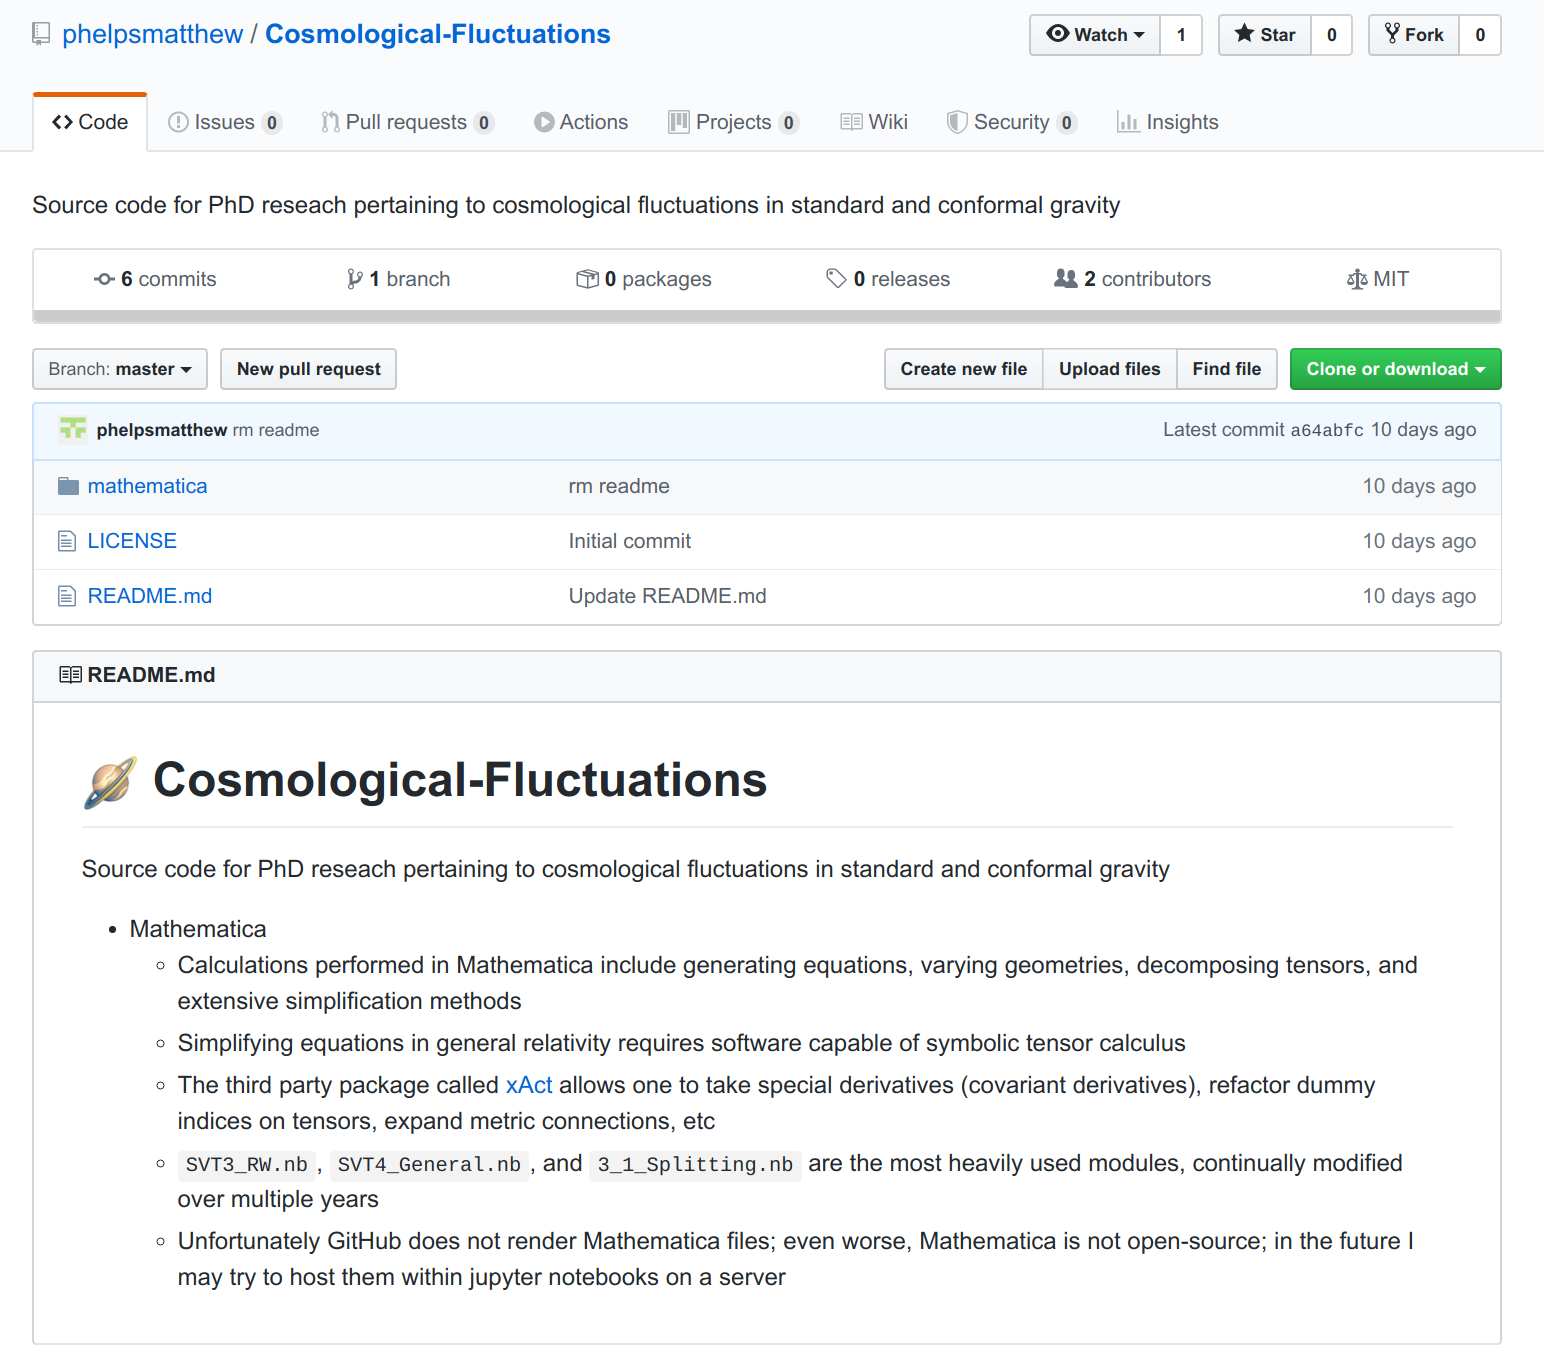
\includegraphics[width=\linewidth]{github.png}
		\end{column}
	\end{columns}
\end{frame}

%%%%%%%%%%%%%%%%%%%%%%%%%%%%%%%%%%%%%%%%%%%%%%%%%%%%%%%%%%%%%%
% Slide  - References
%%%%%%%%%%%%%%%%%%%%%%%%%%%%%%%%%%%%%%%%%%%%%%%%%%%%%%%%%%%%%%

\begin{frame}{References}
		\bibliography{bibliography.bib}
\end{frame}

%%%%%%%%%%%%%%%%%%%%%%%%%%%%%%%%%%%%%%%%%%%%%%%%%%%%%%%%%%%%%%
% Slide  - Acknowledgments
%%%%%%%%%%%%%%%%%%%%%%%%%%%%%%%%%%%%%%%%%%%%%%%%%%%%%%%%%%%%%%

\begin{frame}{Acknowledgments}
	\begin{figure}
		
\includegraphics[width=0.35\linewidth]{network.png}
	\end{figure}
	\let\thefootnote\relax\footnotetext{@bmunst https://link.medium.com/XQlAClsqJ6}
\end{frame}

%%%%%%%%%%%%%%%%%%%%%%%%%%%%%%%%%%%%%%%%%%%%%%%%%%%%%%%%%%%%%%
% Slide  - End
%%%%%%%%%%%%%%%%%%%%%%%%%%%%%%%%%%%%%%%%%%%%%%%%%%%%%%%%%%%%%%

\begin{frame}{}
	\begin{center}
		\Large{The End}
	\end{center}
\end{frame}

%-%-%-%-%-%-%-%-%-%-%-%-%-%-%-%-%-%-%-%-%-%-%-%-%-%-%-%-%-%-%-
%-%-%-%-%-%-%-%-%-%-%-%-%-%-%-%-%-%-%-%-%-%-%-%-%-%-%-%-%-%-%-
%%%%%%%%%%%%%%%%%%%%%%%%%%%%%%%%%%%%%%%%%%%%%%%%%%%%%%%%%%%%%%
\appendix
%%%%%%%%%%%%%%%%%%%%%%%%%%%%%%%%%%%%%%%%%%%%%%%%%%%%%%%%%%%%%%
%-%-%-%-%-%-%-%-%-%-%-%-%-%-%-%-%-%-%-%-%-%-%-%-%-%-%-%-%-%-%-
%-%-%-%-%-%-%-%-%-%-%-%-%-%-%-%-%-%-%-%-%-%-%-%-%-%-%-%-%-%-%-

%%%%%%%%%%%%%%%%%%%%%%%%%%%%%%%%%%%%%%%%%%%%%%%%%%%%%%%%%%%%%%
% Slide  - SVT3 $\delta W_{\mu\nu}$ in Conformal to Flat Backgrounds
%%%%%%%%%%%%%%%%%%%%%%%%%%%%%%%%%%%%%%%%%%%%%%%%%%%%%%%%%%%%%%

\begin{frame}{SVT3 $\delta W_{\mu\nu}$ in Conformal to Flat Backgrounds}
	\begin{eqnarray}
	ds^2 = \Omega^2(x)\bigg[-(1+2\phi)dt^2 + 2(B_i + \tilde\nabla_i B)dt dx^i 
	+ [(1-2\psi)\delta_{ij} + 2\tilde\nabla_i \tilde\nabla_j E + \tilde\nabla_i E_j + \tilde\nabla_j E_i + 2E_{ij}]dx^i dx^j\bigg]
	\end{eqnarray}
	\begin{itemize}
		\item Fluctuation Equations $\delta W_{\mu\nu} = 0$, $\alpha=\phi + \psi +\dot{B}-\ddot{E}$
		\begin{eqnarray}
		\delta W_{00}  &=& -\frac{2}{3\Omega^2} \tilde{\nabla}_{b}\tilde{\nabla}^{b}\tilde{\nabla}_{a}\tilde{\nabla}^{a}\alpha,
		\nonumber\\	
		\delta W_{0i} &=&  -\frac{2}{3\Omega^2} \tilde{\nabla}_i\tilde{\nabla}^a\tilde{\nabla}_a\partial_0\alpha
		+\frac{1}{2\Omega^2}\left[\tilde{\nabla}_{b}\tilde{\nabla}^b(\tilde{\nabla}_a\tilde{\nabla}^a-\partial_0^2)(B_i - \dot{E}_i)\right],
		\nonumber\\	
		\delta W_{ij}  &=& \frac{1}{3\Omega^2}\bigg{[} \delta_{ij}\tilde{\nabla}_{b}\tilde{\nabla}^b (\partial_0^2 - \tilde{\nabla}_a\tilde{\nabla}^a) 
		+(\tilde{\nabla}_{a}\tilde{\nabla}^a -3\partial_0^2)\tilde{\nabla}_i\tilde{\nabla}_j  
		\bigg{] }\alpha
		\\
		&&+\frac{1}{2\Omega^2}\left[ \left[\tilde{\nabla}_{a}\tilde{\nabla}^a -\partial_0^2\right]\left[\tilde{\nabla}_i   \partial_0(B_j - \dot{E}_j)+ \tilde{\nabla}_j \partial_0(B_i - \dot{E}_i)\right] \right]
		+\frac{1}{\Omega^2}\left[\tilde{\nabla}_a\tilde{\nabla}^a-\partial_0^2\right]^2E_{ij}.
		\nonumber
		\end{eqnarray}
		%
		\item Decouple by applying higher derivatives to vector and tensor components
		\begin{eqnarray}
		- \tfrac{2}{3} \tilde{\nabla}_{b}\tilde{\nabla}^{b}\tilde{\nabla}_{a}\tilde{\nabla}^{a}\alpha=0,
		\qquad
		\tilde\nabla_a \tilde\nabla^a \tilde\nabla_b \tilde\nabla^b\left[\tilde\nabla_c \tilde\nabla^c - \partial_0^2\right]^2E_{ij}=0,
		\nonumber\\
		- \tfrac{1}{2} \tilde{\nabla}_{b}\tilde{\nabla}^{b}\tilde{\nabla}_{a}\tilde{\nabla}^{a}(\overset{..}{B}_{i}-\overset{...}{E}_{i}) + \tfrac{1}{2} \tilde{\nabla}_{c}\tilde{\nabla}^{c}\tilde{\nabla}_{b}\tilde{\nabla}^{b}\tilde{\nabla}_{a}\tilde{\nabla}^{a}(B_{i} -\dot{E}_{i})=0
		\end{eqnarray}
	\end{itemize}
\end{frame}

%%%%%%%%%%%%%%%%%%%%%%%%%%%%%%%%%%%%%%%%%%%%%%%%%%%%%%%%%%%%%%
% Slide  - Relating Conformal Gravity to Einstein Gravity
%%%%%%%%%%%%%%%%%%%%%%%%%%%%%%%%%%%%%%%%%%%%%%%%%%%%%%%%%%%%%%

\begin{frame}{Relating Conformal Gravity to Einstein Gravity}
	\begin{eqnarray}
	ds^2 &=& (\eta_{\mu\nu} + h_{\mu\nu})dx^\mu dx^\nu
	\nonumber\\ \nonumber\\
	\delta W_{\mu\nu}&=&\tfrac{1}{2} \nabla_{\beta}\nabla^{\beta}\nabla_{\alpha}\nabla^{\alpha}h_{\mu \nu}
	-  \tfrac{1}{6} g_{\mu \nu} \nabla_{\beta}\nabla^{\beta}\nabla_{\alpha}\nabla^{\alpha}h
	+ \tfrac{1}{6} g_{\mu \nu} \nabla_{\gamma}\nabla^{\gamma}\nabla_{\beta}\nabla_{\alpha}h^{\alpha \beta}
	-  \tfrac{1}{2} \nabla_{\mu}\nabla_{\beta}\nabla^{\beta}\nabla_{\alpha}h_{\nu}{}^{\alpha}
	\nonumber\\
	&& -  \tfrac{1}{2} \nabla_{\nu}\nabla_{\beta}\nabla^{\beta}\nabla_{\alpha}h_{\mu}{}^{\alpha}
	+ \tfrac{1}{6} \nabla_{\nu}\nabla_{\mu}\nabla_{\alpha}\nabla^{\alpha}h
	+ \tfrac{1}{3} \nabla_{\nu}\nabla_{\mu}\nabla_{\beta}\nabla_{\alpha}h^{\alpha \beta}
	\nonumber\\\nonumber\\
	\delta G_{\mu\nu}&=&\tfrac{1}{2} \nabla_{\alpha}\nabla^{\alpha}h_{\mu \nu}
	-  \tfrac{1}{2} g_{\mu \nu} \nabla_{\alpha}\nabla^{\alpha}h
	+ \tfrac{1}{2} g_{\mu \nu} \nabla_{\beta}\nabla_{\alpha}h^{\alpha \beta}
	-  \tfrac{1}{2} \nabla_{\mu}\nabla_{\alpha}h_{\nu}{}^{\alpha}
	-  \tfrac{1}{2} \nabla_{\nu}\nabla_{\alpha}h_{\mu}{}^{\alpha}
	+ \tfrac{1}{2} \nabla_{\nu}\nabla_{\mu}h
	\nonumber\\\nonumber\\
	\delta G &=&  \nabla^\alpha \nabla^\beta h_{\alpha\beta} - \nabla_\alpha\nabla^\alpha h
	\nonumber\\\nonumber\\
	\delta G^{T\theta}_{\mu\nu} &=& \delta G_{\mu\nu} - \frac{1}{3}g_{\mu\nu}\delta G + \frac{1}{3}\nabla_\mu\nabla_\nu \int D \delta G
	\nonumber\\ \nonumber\\
	\nabla^2\delta  G^{T\theta}_{\mu\nu} &=& \nabla^2 \delta G_{\mu\nu} + \frac{1}{3}\left[ 
	\nabla_\mu\nabla_\nu - g_{\mu\nu}\nabla^2\right]\delta G
	\nonumber\\ \nonumber\\
	\nabla^2 \delta G_{\mu\nu}^{T\theta} 
	&=& \tfrac{1}{2} \nabla_{\beta}\nabla^{\beta}\nabla_{\alpha}\nabla^{\alpha}h_{\mu \nu}
	-  \tfrac{1}{6} g_{\mu \nu} \nabla_{\beta}\nabla^{\beta}\nabla_{\alpha}\nabla^{\alpha}h
	+ \tfrac{1}{6} g_{\mu \nu} \nabla_{\gamma}\nabla^{\gamma}\nabla_{\beta}\nabla_{\alpha}h^{\alpha \beta}
	-  \tfrac{1}{2} \nabla_{\mu}\nabla_{\beta}\nabla^{\beta}\nabla_{\alpha}h_{\nu}{}^{\alpha}
	\nonumber\\
	&& -  \tfrac{1}{2} \nabla_{\nu}\nabla_{\beta}\nabla^{\beta}\nabla_{\alpha}h_{\mu}{}^{\alpha}
	+ \tfrac{1}{6} \nabla_{\nu}\nabla_{\mu}\nabla_{\alpha}\nabla^{\alpha}h
	+ \tfrac{1}{3} \nabla_{\nu}\nabla_{\mu}\nabla_{\beta}\nabla_{\alpha}h^{\alpha \beta}
	\nonumber\\
	&=& \delta W_{\mu\nu}
	\end{eqnarray}
\end{frame}

\end{document}
%%%%%%%%%%%%%%%%%%%%%%%%%%%%%%%%%%%%%%%%%%%%%%%%%%%%%%%%%%%%%%
% End Document
%%%%%%%%%%%%%%%%%%%%%%%%%%%%%%%%%%%%%%%%%%%%%%%%%%%%%%%%%%%%%%